\documentclass[13pt]{scrreprt}
\usepackage[utf8]{inputenc} % use utf8 file encoding for TeX sources
\usepackage[T1]{fontenc}    % avoid garbled Unicode text in pdf
\usepackage[german]{babel}  % german hyphenation, quotes, etc
\usepackage{hyperref}       % detailed hyperlink/pdf configuration
\usepackage{graphicx}       % provides com\dfrac{m}{Nenner}ands for including figures
\usepackage{csquotes}       % provides \enquote{} macro for "quotes"
\usepackage[nonumberlist]{glossaries}     % provides glossary commands
\usepackage{enumitem}
\usepackage[center]{caption}
\usepackage[export]{adjustbox}
\newcounter{tempcounter1}
\newcounter{tempcounter2}
\newcounter{tempcounter3}
\newcounter{tempcounter4}
\newcounter{tempcounter5}
\newcounter{tempcounter6}
\newcounter{tempcounter7}
\newcounter{tempcounter8}
\newcounter{tempcounter9}

\makenoidxglossaries

\newglossaryentry{unterschiedlich}
{
	name=unterschiedlich,
	description={Sei $G=(V,E)$ ein einfacher Graph, $C$ eine endliche Menge an Farben und $c_1: V \rightarrow C$ sowie $c_2: V \rightarrow C$ F\"arbungen. $c_1$ und $c_2$ heißen unterschiedlich, wenn keine Abbildung $p: C \rightarrow C$ existiert, sodass $p \circ c_1 = c_2$.
	Analog für totale F\"arbungen $c_1: V \times E \mapsto C$ und $c_2: V \times E \mapsto C$}
}
\newglossaryentry{Totalfaerbungsvermutung}
{
	name=Totalfärbungsvermutung,
	description={Sei $G=(V,E)$ ein einfacher Graph und $C$ eine endliche Menge an Farben. Eine Totalfärbung $c: V \times E \mapsto C$ ist gültig, wenn adjazente und inzidente Elemente unterschiedliche Farben haben, wenn also Folgendes gilt:
	$$  \forall v_i, v_j \in V: ((v_i, v_j) \in E \rightarrow c(v_i) \neq c(v_j)) $$
	$$  \forall v \in V, e=(v_1, v_2) \in E: (v \in \{v_1, v_2\} \rightarrow c(v) \neq c(e)) $$
	Die minimale Anzahl an Farben, die für eine gültige Totalfärbung von $G$ nötig ist, heißt totalchromatische Zahl $\chi (G)$. 
	Die Totalfärbungsvermutung besagt, dass
	 $$ \chi (G) \leq \Delta (G) + 2 $$
	 wobei $\Delta (G)$ den maximalen Knotengrad in $G$ bezeichnet
	}
}
\newglossaryentry{Subgraph}
{
	name=Subgraph,
	description={Wenn man von einem Graphen Kanten beziehungsweise Knoten entfernt und den restlichen Graphen unberührt lässt, erhält man einen Subgraphen des Orginalgraphen}
}
\newglossaryentry{Merkmal}
{
	name=Merkmal,
	description={Als Merkmale werden hier Kanten- sowie Knotenanzahl eines Graphen und die Werte, welche von den in \ref{FA6} angegebenen Algorithmen berechnet werden, betrachtet},
	plural=Merkmale
}
\newglossaryentry{Filter}
{
	name=Filter,
	description={Filter wird auf \Glspl{Merkmal} der Graphen angewendet. Graphen, welche die ausgewählten Filterbedingungen erfüllen, werden ausgewählt}
}


\title{
	
\includegraphics[scale=0.5,center]{OfficialLogo.png}
	\\
	Pflichtenheft
}
\author{\\ \\ \\ \\ Marijan Petričević, Christoph Hartmann, Clara Walendy,\\
	 Jakob Dräger, Julius Meißner}

\begin{document}
\maketitle

% Platzierung des Inhaltsverzeichnisses
\tableofcontents

\chapter{Motivation}

Dieses Pflichtenheft ist im Rahmen des Pflichtmoduls Praxis der Softwareentwicklung des
Bachelor-Studiengangs Informatik am Karlsruher Institut für Technologie entstanden. Das
Projekt wurde am Lehrstuhl für Systeme der Informationsverwaltung angeboten.
\newline
\ \\
Graphitty soll die Forschung in der Graphentheorie erleichtern. Die Software soll einen Forscher dabei unterstützen Korrelationen zwischen Merkmalen von Graphen und der Totalfärbungsvermutung zu finden. \newline
\ \\
Die Totalfärbungsvermutung ist ein offenes Problem der Informatik. Die Vermutung ist bisher nur für einige Graphklassen gezeigt worden. Eine wichtige Rolle spielt dabei das Totalfärbungsproblem.\\
Bei dem Totalfärbungsproblem soll ein Graph so eingefärbt werden, dass benachbarte Knoten und  benachbarte Kanten nicht dieselbe Farbe haben. Außerdem sollen Knoten nicht diesselbe Farbe haben, wie die Kanten, die an ihnen enden.\\
Da bei dichteren Graphen zum Beispiel prozentual mehr Knoten und Kanten zusammen hängen, ist zu vermuten, dass dieses Merkmal in Zusammenhang mit Graphenfärbung steht. \\
Dieser und andere potentielle Zusammenhänge sollen nun durch das Produkt mithilfe von rechnergestützter Graphengenerierung und Merkmalsberechnung untersucht werden können.


\chapter{Zielbestimmung}

Der Anwender wird durch das Produkt in die Lage versetzt, zufällig generierte Graphen auf Zusammenhänge zwischen \Glspl{Merkmal}n die die Struktur und die Färbbarkeit des Graphen betreffen, zu überprüfen. Im Folgenden wird der Ablauf des Programms, unterteilt in Muss- und Kannkriterien anhand den Unterpunkten Graphengenerierung, \Gls{Merkmal}sberechnung, Graphenspeicherung, Datenbankauswertung und Benutzeroberfläche erläutert.

\section{Musskriterien}

\subsection{Graphengenerierung}
	\begin{itemize} [label={}]
	\item Die Graphen sollen randomisiert generiert werden. Der Status dieses Prozesses ist über eine Textausgabe in der Benutzeroberfläche verfolgbar.
	\item Die maximale Knotenanzahl der zu generierenden Graphen ist durch den Nutzer einstellbar.
	\end{itemize}
	
\subsection{Graphenanalyse}
	\begin{itemize} [label={}]
	\item Für die generierten Graphen sollen verschiedene \Glspl{Merkmal}, wie zum Beispiel die totalchromatische Zahl und Dichte des Graphen überprüft und berechnet werden. \\ Eine genaue Ausführung aller zu berechnenden \Glspl{Merkmal} findet sich in den funktionalen Anforderungen unter \ref{FA6}. 
	\end{itemize}
	
\subsection{Graphenspeicherung}
	\begin{itemize} [label={}]
	\item Sobald alle \Glspl{Merkmal} eines Graphen bestimmt wurden, wird der Graph mit seinen \Glspl{Merkmal}n in eine Datenbank zur späteren Abfrage eingespeichert. Außerdem sollen durch den Benutzer modifizierte (Spezifikation siehe \ref{FA202}) Graphen ebenfalls wieder in die Datenbank eingepflegt werden. 
	\end{itemize}

\subsection{Datenbankauswertung}
	\begin{itemize} [label={}]
	\item Auf die oben angesprochene Datenbank, soll der Benutzer nun anhand von Kriterien, wie zum Beispiel die zehn dichtesten Graphen, zugreifen können. Es werden dann die entsprechenden Graphen in einer Liste aufgeführt. Außerdem werden Graphen mit den extremsten Merkmalsausprägungen hervorgehoben. Um spezifischere Anfragen zu ermöglichen, soll der Benutzer die Suchkriterien auch kombinieren können.
	\end{itemize}

\subsection{Benutzeroberfläche}
\subsubsection{Graphenvisualisierung}
	\begin{itemize}[label={}]
    	\item Die Auswahl an Graphen, die den vom Nutzer gewählten Kriterien entsprechen, werden in einer Übersicht dargestellt. 
	\end{itemize}

\subsubsection{Graphvisualisierung}
	\begin{itemize}[label={}]
    	\item Ein, aus der oben beschriebenen Übersicht vom Nutzer ausgewählter Graph soll in seiner strukturellen Gesamtheit angezeigt werden können. Dann kann der Graph, falls gewünscht durch Hinzufügen beziehungsweise Entfernen von Knoten oder Kanten geringfügig bearbeitet werden.
	\end{itemize}

\section{Kannkriterien}

\subsection{Graphengenerierung}
	\begin{itemize}[label={}]
	\item Zu einem gewählten Graphen lässt sich der nächst dichteren Graph generieren.
	\end{itemize}

\subsection{Graphenvisualisierung}
	\begin{itemize}[label={}]
	\item Die Anwendung listet nach der Generierung alle Graphen mit den extremsten Merkmalen in der Übersicht auf, um den Zugriff auf die potentiell interessantesten Graphen schnell zu ermöglichen.
	\end{itemize}


\section{Abgrenzungskriterien}

\subsection{Funktionalität}
	\begin{itemize}[label={}]
	\item Die maximale Knotenzahl der generierten Graphen ist 20.
	\item Die Anwendung garantiert keine neuen Erkenntnisse in der Graphentheorie.
	\end{itemize}

\subsection{Produktumgebung}
	\begin{itemize}[label={}]
	\item Das Produkt muss nur auf einem PC mit Windows Betriebssystem ausführbar sein.
	\item Das Produkt muss nicht mit mobilen Endgeräten kompatibel sein.
	\end{itemize}

\subsection{Benutzerfreundlichkeit}
	\begin{itemize}[label={}]
	\item Die Sprache des Produkts ist ausschließlich Englisch.
	\item Das Produkt muss nicht barrierefrei sein.
	\end{itemize}



\chapter{Produkteinsatz}

\section{Anwendungsbereich}
	\begin{itemize}[label={}]
	\item{Das Produkt unterstützt die Forschung im Bereich der Graphentheorie, bezüglich des Problems der \Gls{Totalfaerbungsvermutung}, in dem es zufällige Graphen generiert und diese aufbereitet zur Analyse darstellt.}
	\end{itemize}

\section{Zielgruppe}
	\begin{itemize}[label={}]
	\item{Die Zielgruppe sind Wissenschaftler, die im Bereich der Graphentheorie arbeiten, über grundlegende Kenntnisse im Umgang mit Software verfügen und Englisch verstehen.}
	\end{itemize}

\section{Betriebsbedingungen}
	\begin{itemize}[label={}]
	\item{Die Software soll in geschlossenen Arbeitsräumen und bei kontinuierlicher Stromversorgung verwendet werden. Die Stromversorgung ist vor allem bei längeren Graphen-Generierungsprozessen notwendig, um korrumpierte Elemente in der Datenbank zu vermeiden.}
	\end{itemize}



\chapter{Produktumgebung}

Die Anwendung ist ein Windows-Programm mit Anbindung an einen Hintergrundspeicher.

\section{Software}
\begin{itemize}
	\item{Auf dem PC muss Windows 7\footnote{https://www.microsoft.com/de-de/software-download/windows7} oder neuer installiert sein.}
	\item{Das .NET Framework\footnote{https://www.microsoft.com/de-DE/download/details.aspx?id=30653}, in der Version 4.5 oder neuer, muss installiert sein.}
\end{itemize}

\section{Hardware}
\begin{itemize}
	\item{Die Zielplattform ist ein Windows-PC.}
	\item{Zum Speichern auf einer Remote-Datenbank ist eine funktionierende Netzwerkanbindung erforderlich.}
\end{itemize}

\section{Produktschnittstellen}
\begin{itemize}
\item{Zum Verwalten von Daten wird ein MariaDB\footnote{https://mariadb.org/download/} Datenbankmanagementsystem verwendet.}
\end{itemize}

\chapter{Funktionale Anforderungen}

\section{Grundfunktionalität}
\subsection{Musskriterien}
\begin{addmargin}[25pt]{0pt}
\begin{enumerate} [label=FA\arabic*,start=100]
	\item \label{FA100}Die Anwendung wartet nach dem Starten auf Benutzereingaben.
	\item \label{FA101}Die Datenbank wird beim ordnungsgemäßen Schließen der Anwendung gesichert.
\setcounter{tempcounter3}{\value{enumi}}
\end{enumerate}
\end{addmargin}
\addtocounter{tempcounter3}{1}
%\subsection{Kannkriterien}
\begin{addmargin}[25pt]{0pt}
\begin{enumerate} [label=FA\arabic*,start=\value{tempcounter3}]
%Kannkriterien hier
\end{enumerate}
\end{addmargin}

\section{Datenbank}
\subsection{Musskriterien}
\begin{addmargin}[25pt]{0pt}
\begin{enumerate} [label=FA\arabic*,start=200]
	\item \label{FA200}Die generierten Graphen werden nach der Anwendung der Algorithmen mit ihren \Glspl{Merkmal}n in einer Datenbank gespeichert.
	\item \label{FA201}Es können Graphen samt den dazu gespeicherten \Glspl{Merkmal}n gelöscht werden.
	\item \label{FA202}In einem beliebig ausgewähltem Graphen können Kanten entfernt oder hinzugefügt werden.
	\item \label{FA203}Für den in \ref{FA202} modifizierten Graphen können die \Glspl{Merkmal} neu berechnet werden.
	\item \label{FA204}Der in \ref{FA202} und \ref{FA203} beschriebene Graph kann anschließend wieder in die Datenbank eingepflegt werden.
    \item \label{FA205}Die Datenbank muss vom Datenbankmanagementsystem MariaDB verwaltbar sein können.
\setcounter{tempcounter4}{\value{enumi}}
\end{enumerate}
\end{addmargin}
\addtocounter{tempcounter4}{1}
%\subsection{Kannkriterien}
%\begin{addmargin}[25pt]{0pt}
%\begin{enumerate}[label=FA\arabic*,start=\value{tempcounter4}]
%\end{enumerate}
%\end{addmargin}
%Auskommentiert, weil es momentan nicht gebraucht wird, man es in der Zukunft aber vielleicht braucht...Außerdem Kommentar in Deutsch, weil ich müde bin ~Clara

\section{Graphengenerierung}
\subsection{Musskriterien}
\begin{addmargin}[25pt]{0pt}
\begin{enumerate} [label=FA\arabic*,start=300]
	\item \label{FA300}Die Graphen werden zufallsbasiert generiert.
	\item Standardmäßig werden Graphen mit einer Anzahl von 20 Knoten generiert.
	\item Vor der Generierung soll es möglich sein eine eigene Anzahl von Knoten festzulegen.
\setcounter{tempcounter5}{\value{enumi}}
\end{enumerate}
\end{addmargin}

\addtocounter{tempcounter5}{1}
\subsection{Kannkriterien}
\begin{addmargin}[25pt]{0pt}
\begin{enumerate}[label=FA\arabic*,start=\value{tempcounter5}]
	\item Zu dem im Moment gewählten Graphen lässt sich der nächst dichtere Graph generieren.
	\item Für jeden generierten Graphen kann zusätzlich der nächst dichtere Graph generiert werden.
	\item Für einen Graphen lässt sich sukzessive der nächst dichtere Graph bestimmen.
\end{enumerate}
\end{addmargin}


\section{Grafische Benutzeroberfläche}
\subsection{Musskriterien}
\begin{addmargin}[25pt]{0pt}
\begin{enumerate} [label=FA\arabic*,start=400]
	\item \label{FA400}Durch Anwendung von Filtern soll es möglich sein, Graphen die diesen Filterkriterien entsprechen übersichtlich darzustellen. Dabei kann über alle in \ref{FA6} und folgende angegebenen \Glspl{Merkmal} gefiltert werden.	
	\item \label{FA401}Die in \ref{FA400} genannten Filter sollen kombinatorisch anwendbar sein.
	\item Es sollen die n am stärksten korrellierenden Merkmale angezeigt werden.
	\item Korrelationen zwischen den verschiedenen \Glspl{Merkmal}n sollen verdeutlicht werden, sofern die Merkmale stark korrelieren.
\setcounter{tempcounter6}{\value{enumi}}
\end{enumerate}
\end{addmargin}

\addtocounter{tempcounter6}{1}
\subsection{Kannkriterien}
\begin{addmargin}[25pt]{0pt}
\begin{enumerate} [label=FA\arabic*,start=\value{tempcounter6}]
		\item Falls Graphen-\Glspl{Merkmal} Extremwerte annehmen, sollen diese gesondert hervorgehoben werden.
		\item Nachdem alle Graphen generiert wurden, werden diejenigen mit den extremsten Werten in der Übersicht dargestellt.
		\item Filterkonfigurationen sollen gespeichert werden können.
\end{enumerate}
\end{addmargin}


\section{Darstellung der Graphen}
\subsection{Musskriterien}
\begin{addmargin}[25pt]{0pt}
\begin{enumerate} [label=FA\arabic*,start=500]
	\item \label{FA500}Der generierte Graph soll dargestellt werden, indem die Knoten und Kanten grafisch angezeigt werden.
	\item Existiert eine gültige Färbung, so wird diese dargestellt.
	\item Die berechneten \Glspl{Merkmal} sollen angezeigt werden.
\setcounter{tempcounter7}{\value{enumi}}
\end{enumerate}
\end{addmargin}
\addtocounter{tempcounter7}{1}
\subsection{Kannkriterien}
\begin{addmargin}[25pt]{0pt}
\begin{enumerate} [label=FA\arabic*,start=\value{tempcounter7}]
	\item \label{FA503}Es soll eine Zoom-Funktion geben, mit der Ausschnitte des Graphen betrachtet werden können. 
	\item \label{FA504}Bei einer Detaildarstellung soll es möglich sein, den Ausschnitt zu bewegen, um andere Teile des Graphen sichtbar zu machen.
\end{enumerate}
\end{addmargin}

\newpage
\section{Graphenanalyse}
\label{Graphenanalyse}
\subsection{Musskriterien}
Nachdem ein Graph generiert wird, werden folgende Merkmale bestimmt, beziehungsweise berechnet. \\
\begin{addmargin}[25pt]{0pt}
\begin{enumerate} [label=FA\arabic*,start=600]
	\label{FA6}
	\item Anzahl der Knoten $n$
    \item Anzahl der Kanten $m$
	\item Durchschnittlicher Knotengrad $d$
	\item Maximaler Knotengrad $\Delta$
	\item Größe der größten im Graph enthaltenen Clique
	\item Anzahl der Cliquen der Größe $k$ für $3 \leq k \leq n$
	\item Dichte gemäß BFS-Code
	\item Anzahl der Graphen im Datenbestand mit höherer BFS-Dichte, als der betrachtete Graph (ausgehend von gleicher Knotenanzahl).
    \item Dichte gemäß Profil 
	\item Anzahl der Graphen im Datenbestand mit höherer Profil-Dichte, als der betrachtete Graph (ausgehend von gleicher Knotenanzahl).
	\item Ist die \Gls{Totalfaerbungsvermutung} erfüllt?
    \item Totalchromatische Zahl $\chi$
    \item Aufwand, um eine gültige minimale Färbung zu berechnen in Sekunden
    \item Anzahl der Graphen in der Datenbank mit gleicher Knotenanzahl
   	\item Anzahl der Graphen im Datenbestand mit kleinerer oder gleicher totalchromatischer Zahl, als der betrachtete Graph (ausgehend von gleicher Knotenanzahl).
\setcounter{tempcounter8}{\value{enumi}}
\end{enumerate}
\end{addmargin}
\addtocounter{tempcounter8}{1}
\subsection{Kannkriterien}
\begin{addmargin}[25pt]{0pt}
\begin{enumerate} [label=FA\arabic*,start=\value{tempcounter8}]
   	 \item Anzahl unterschiedlicher Totalfärbungen mit $\chi$ Farben
    	
\end{enumerate}
\end{addmargin}



\chapter{Nichtfunktionale Anforderungen}

\section{Erweiterbarkeit}
Eine leichte Erweiterbarkeit des Produkts soll durch folgende Punkte möglich sein. Dabei wird erwartet, dass eine Person mit Kenntnissen in der Programmierung und Datenbankeinsatz diese Erweiterungen vornimmt.
\\
\begin{addmargin}[25pt]{0pt}
\begin{enumerate} [label=NF\arabic*00,start=1]	
	\item Merkmale sollen mit wenig Aufwand hinzugefügt werden können. Dazu müssen mit Hilfe eines Datennbankmanagementsystems entsprechende  Attribute in der Graphen Relation in der Datenbank hinzugefügt werden. Ebenfalls muss im Programmcode ein neues Attribut in der Klasse des Graphen hinzugefügt und eine Berechnung dieses Merkmals implementiert werden.
	\item Neue Dichtedefinitionen sollen ebenfalls leicht einführbar sein. Dazu muss erneut wie vorher beschrieben ein neues Merkmal für den Dichtewert hinzugefügt werden.
	\item Eigene Graphengeneratoren sollen an einer vorgegebenen Stelle implementiert werden können und später im Programm einfach auswählbar sein.
\end{enumerate}
\end{addmargin}

\section{Weitere}
\begin{addmargin}[25pt]{0pt}
\begin{enumerate} [label=NF\arabic*00,start=4]
        \item Das System soll für eine Person mit Programmierkenntnissen leicht zu warten sein. Dazu muss das System u.a. gut dokumentiert sein.
        \item Das System soll über einen längeren Zeitraum (mind. über Nacht) zuverlässig (ohne Abstürze) oder die Notwendigkeit einer Benutzereingabe Graphen generieren und Merkmale berechnen können.
        \item Ein Systemabsturz darf keinen Verlust der bereits berechneten Graphen und Merkmale verursachen.
        \item Das Berechnen der Merkmale eines Graphen soll eine angemessene Zeit- und Speicherkomplexität besitzen. Eine stark optimierte Berechnung ist nicht notwendig.
        \item Die Benutzeroberfläche des Systems sollen zu jeder Zeit auf Benutzereingaben antworten können.
\end{enumerate}
\end{addmargin}


\chapter{Produktdaten}

\section{Zu speichernde Daten}
Folgende Daten sind zu speichern:

\subsection{Graphen}
\begin{addmargin}[25pt]{0pt}
\begin{enumerate} [label=D\arabic*,start=100]
	\item Knoten inklusive der berechneten Färbung
	\item Kanten inklusive der berechneten Färbung
	\item Serialisierte Speicherung der Graphen in der Datenbank
\end{enumerate}
\end{addmargin}

\subsection{Graphenmerkmale}
\begin{addmargin}[25pt]{0pt}
	Sämtliche Merkmale die in den Funktionalen Anforderungen unter dem Abschnitt Graphenanalyse aufgelistet sind, sollen in einer Datenbank statisch abgespeichert werden.
\end{addmargin}

\subsection{Graphenmetadaten}
\begin{addmargin}[25pt]{0pt}
\begin{enumerate} [label=D\arabic*,start=300]
	\item ID des Graphen
\end{enumerate}
\end{addmargin}

\subsection{Nutzerdaten}
\begin{addmargin}[25pt]{0pt}
\begin{enumerate} [label=D\arabic*,start=400]
	\item Filterkonfigurationen des Nutzers
\end{enumerate}
\end{addmargin}


\section{Datenflussdiagramme}

\subsection{Graphengenerierung}
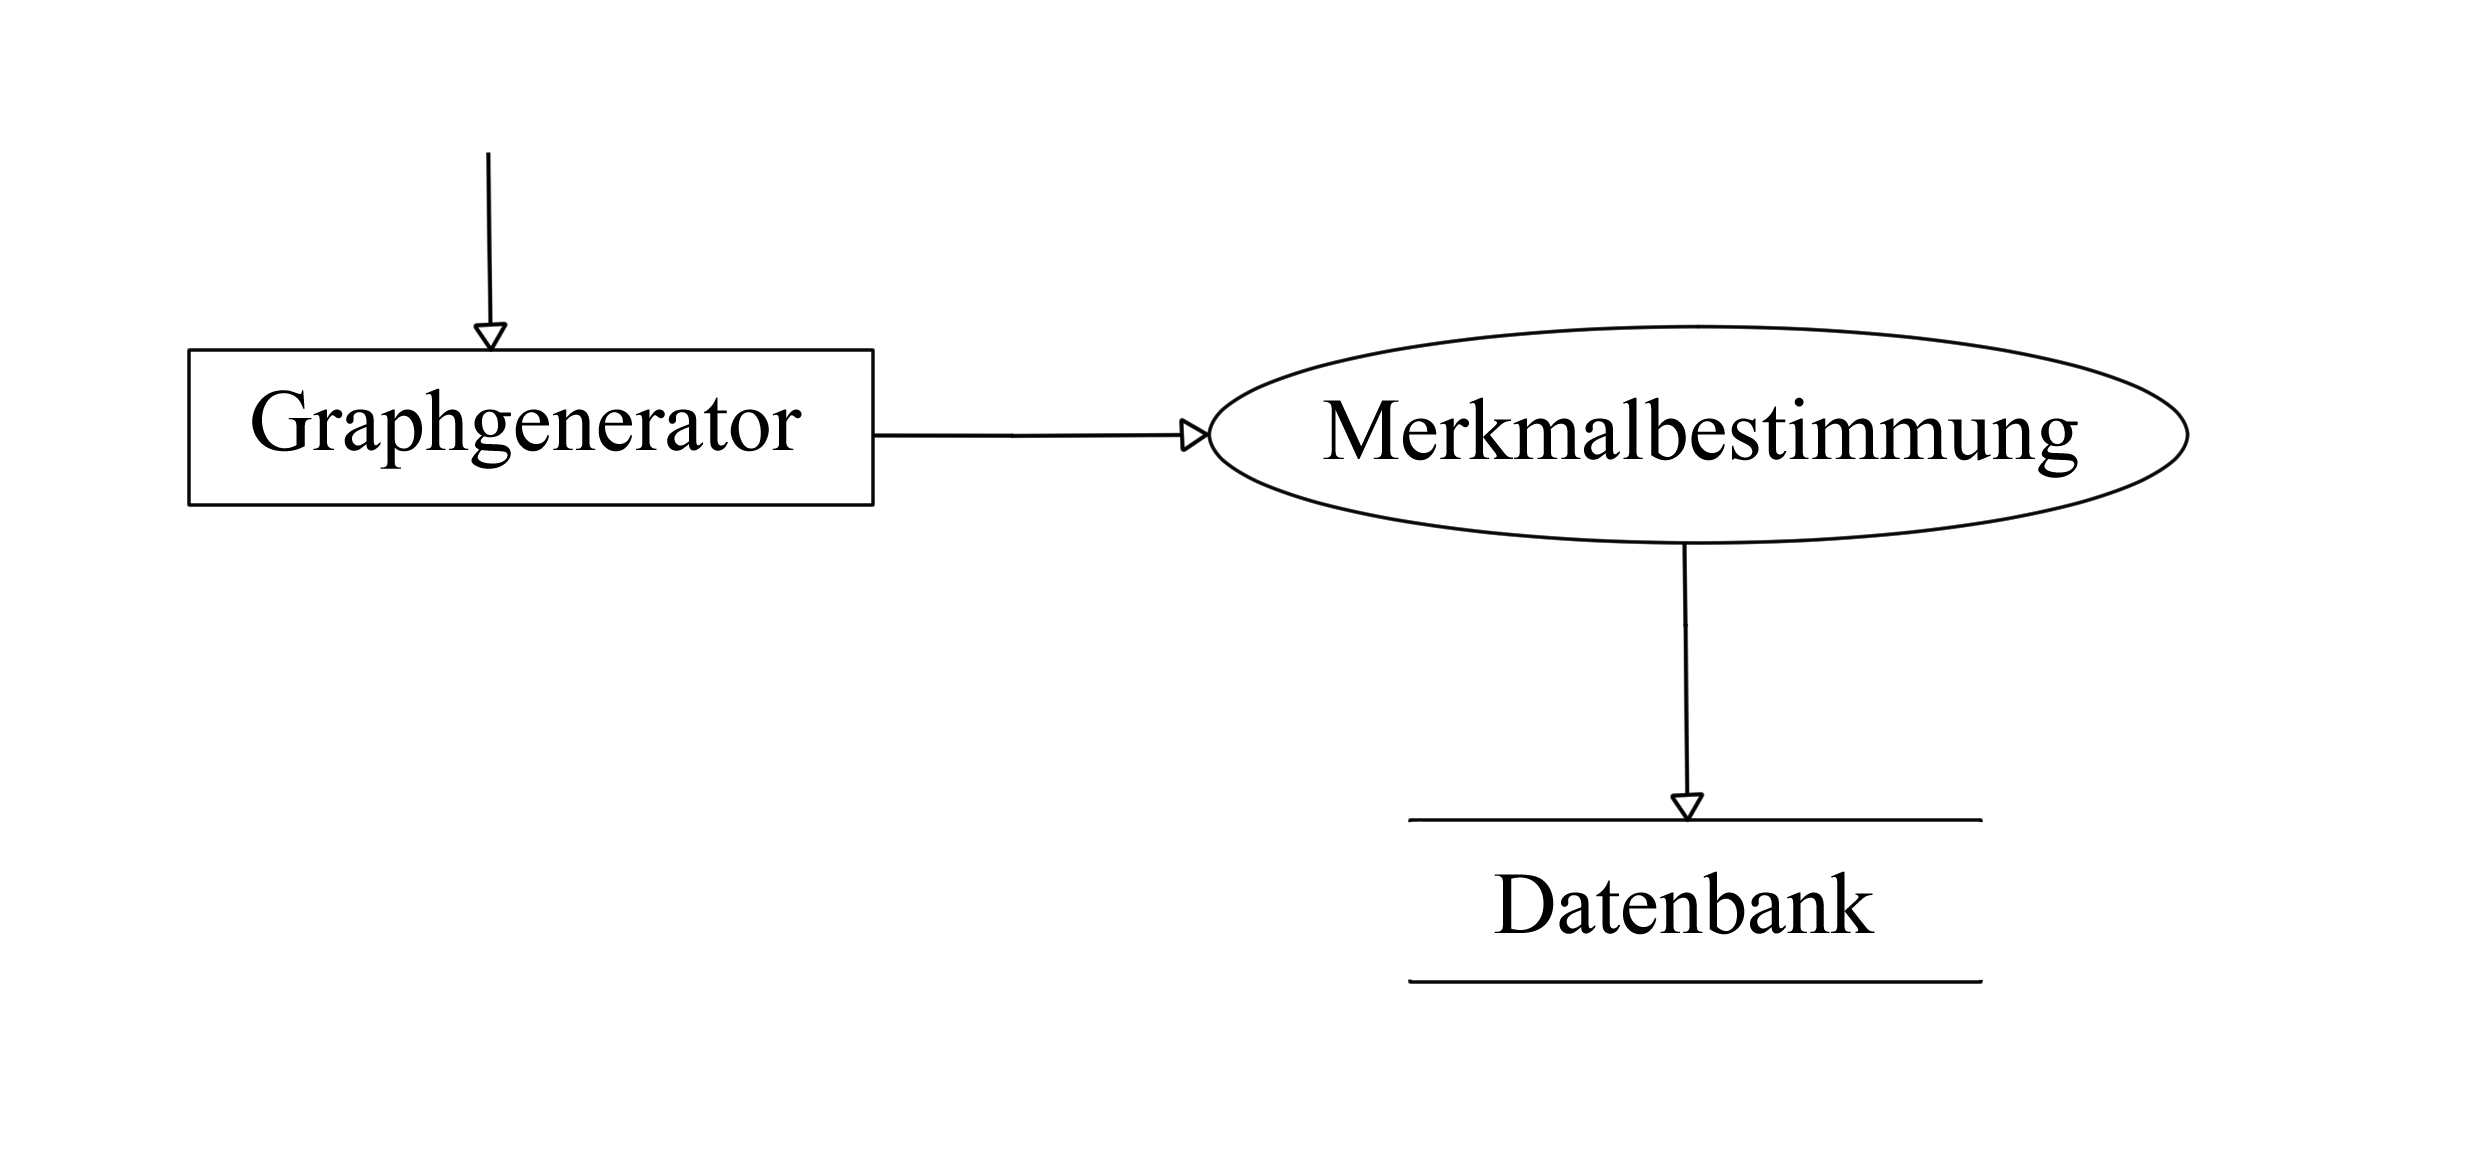
\includegraphics[scale=0.75]{Graphengenerierung_Datenflussdiagramm.jpg}
\\
\\
\\
\subsection{Graphenvisualisierung}
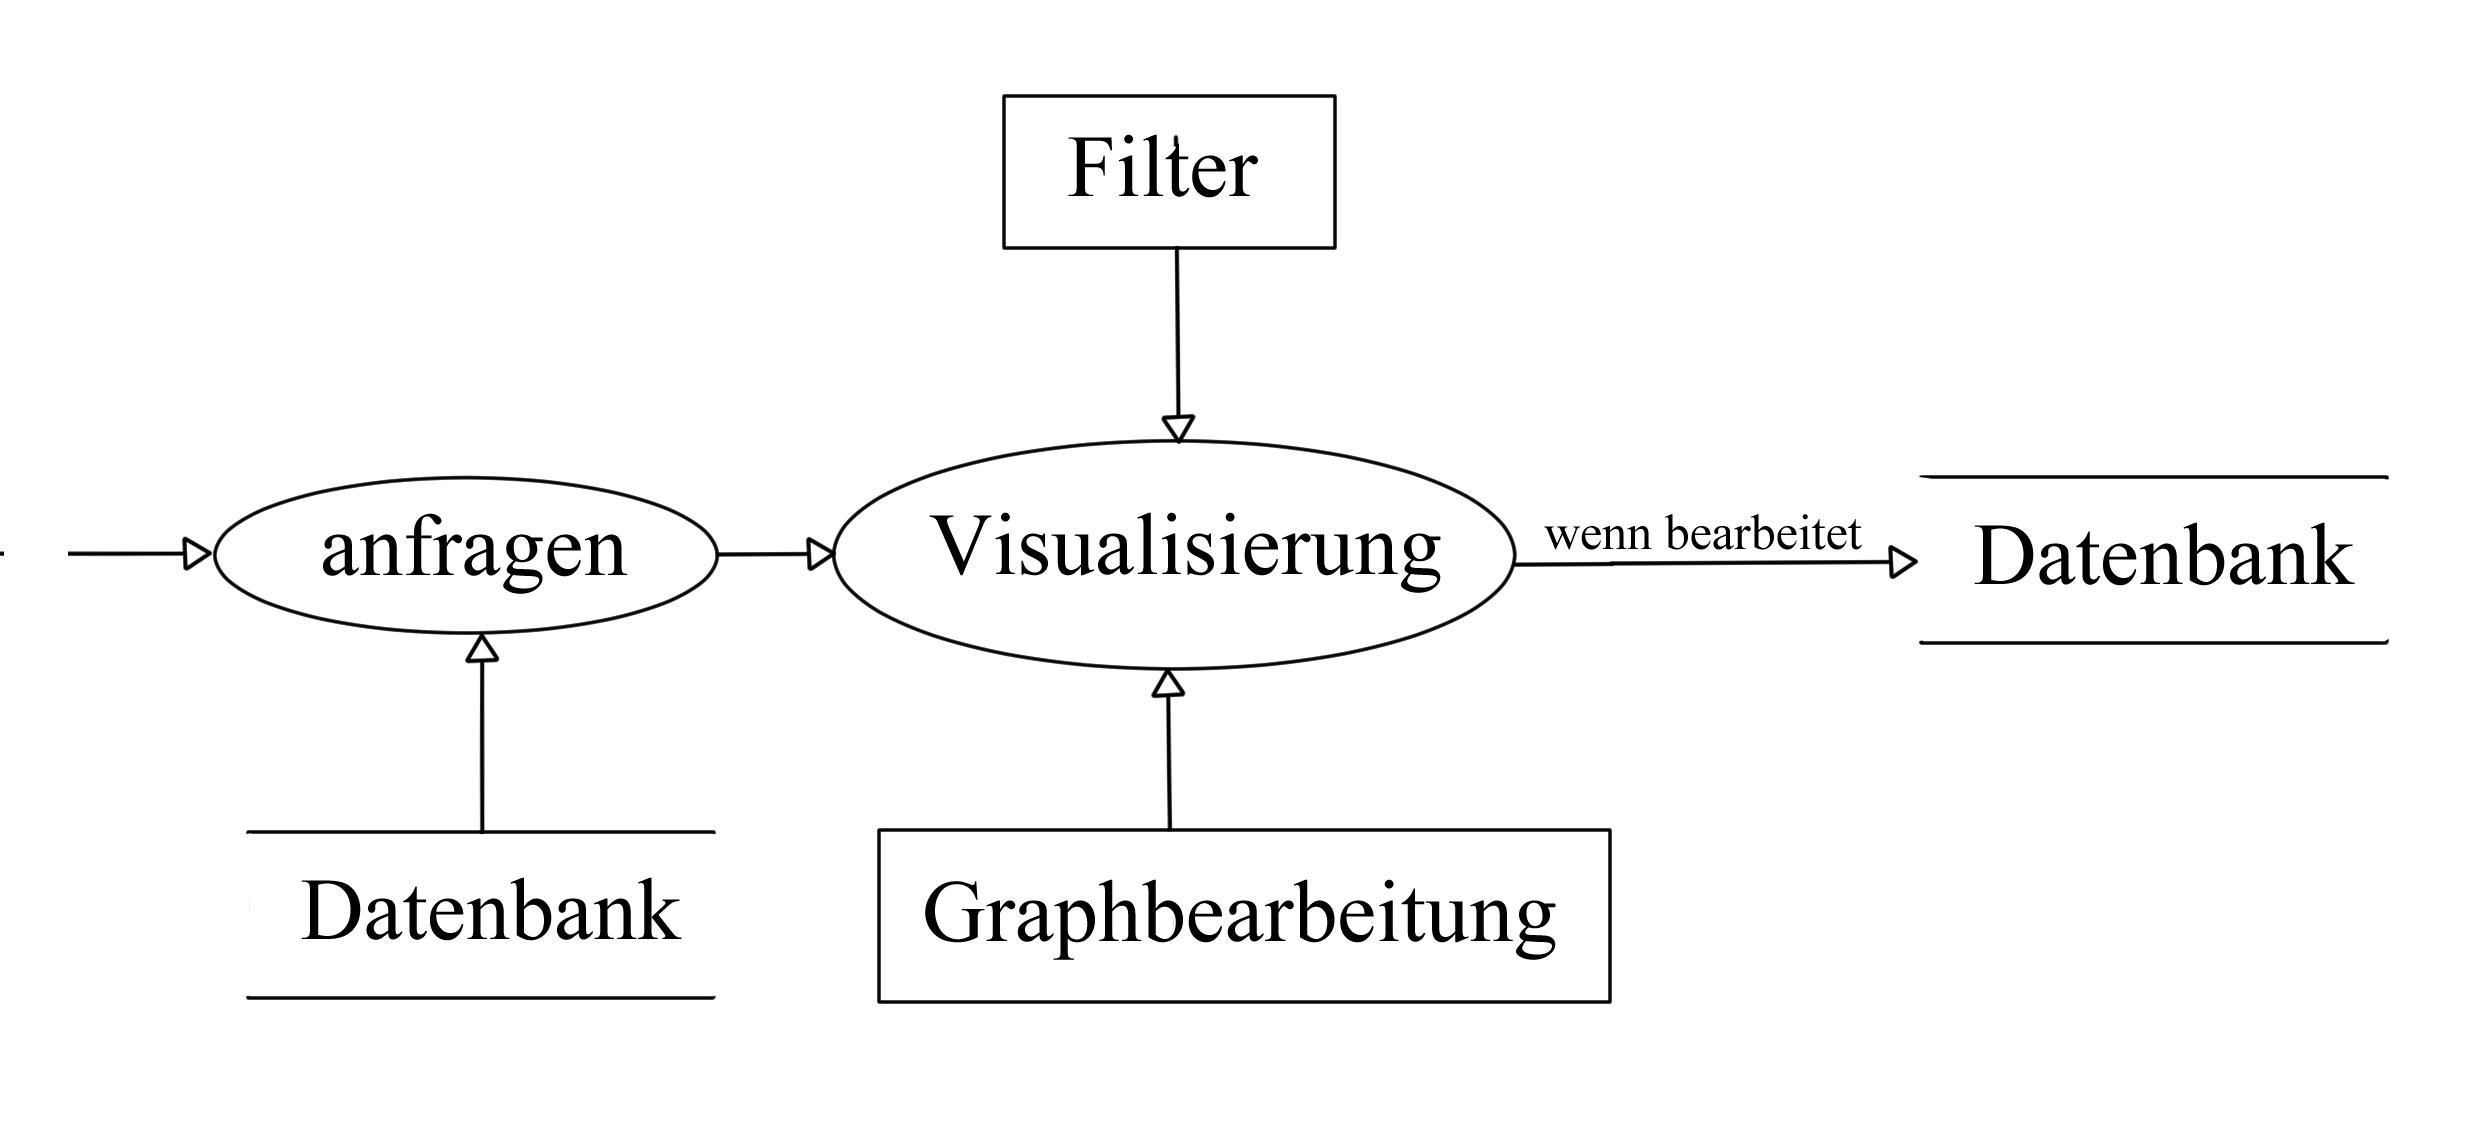
\includegraphics[scale=0.75]{Graphenvisualisierung_Datenflussdiagramm.jpg}

\chapter{Anwendungsfälle}

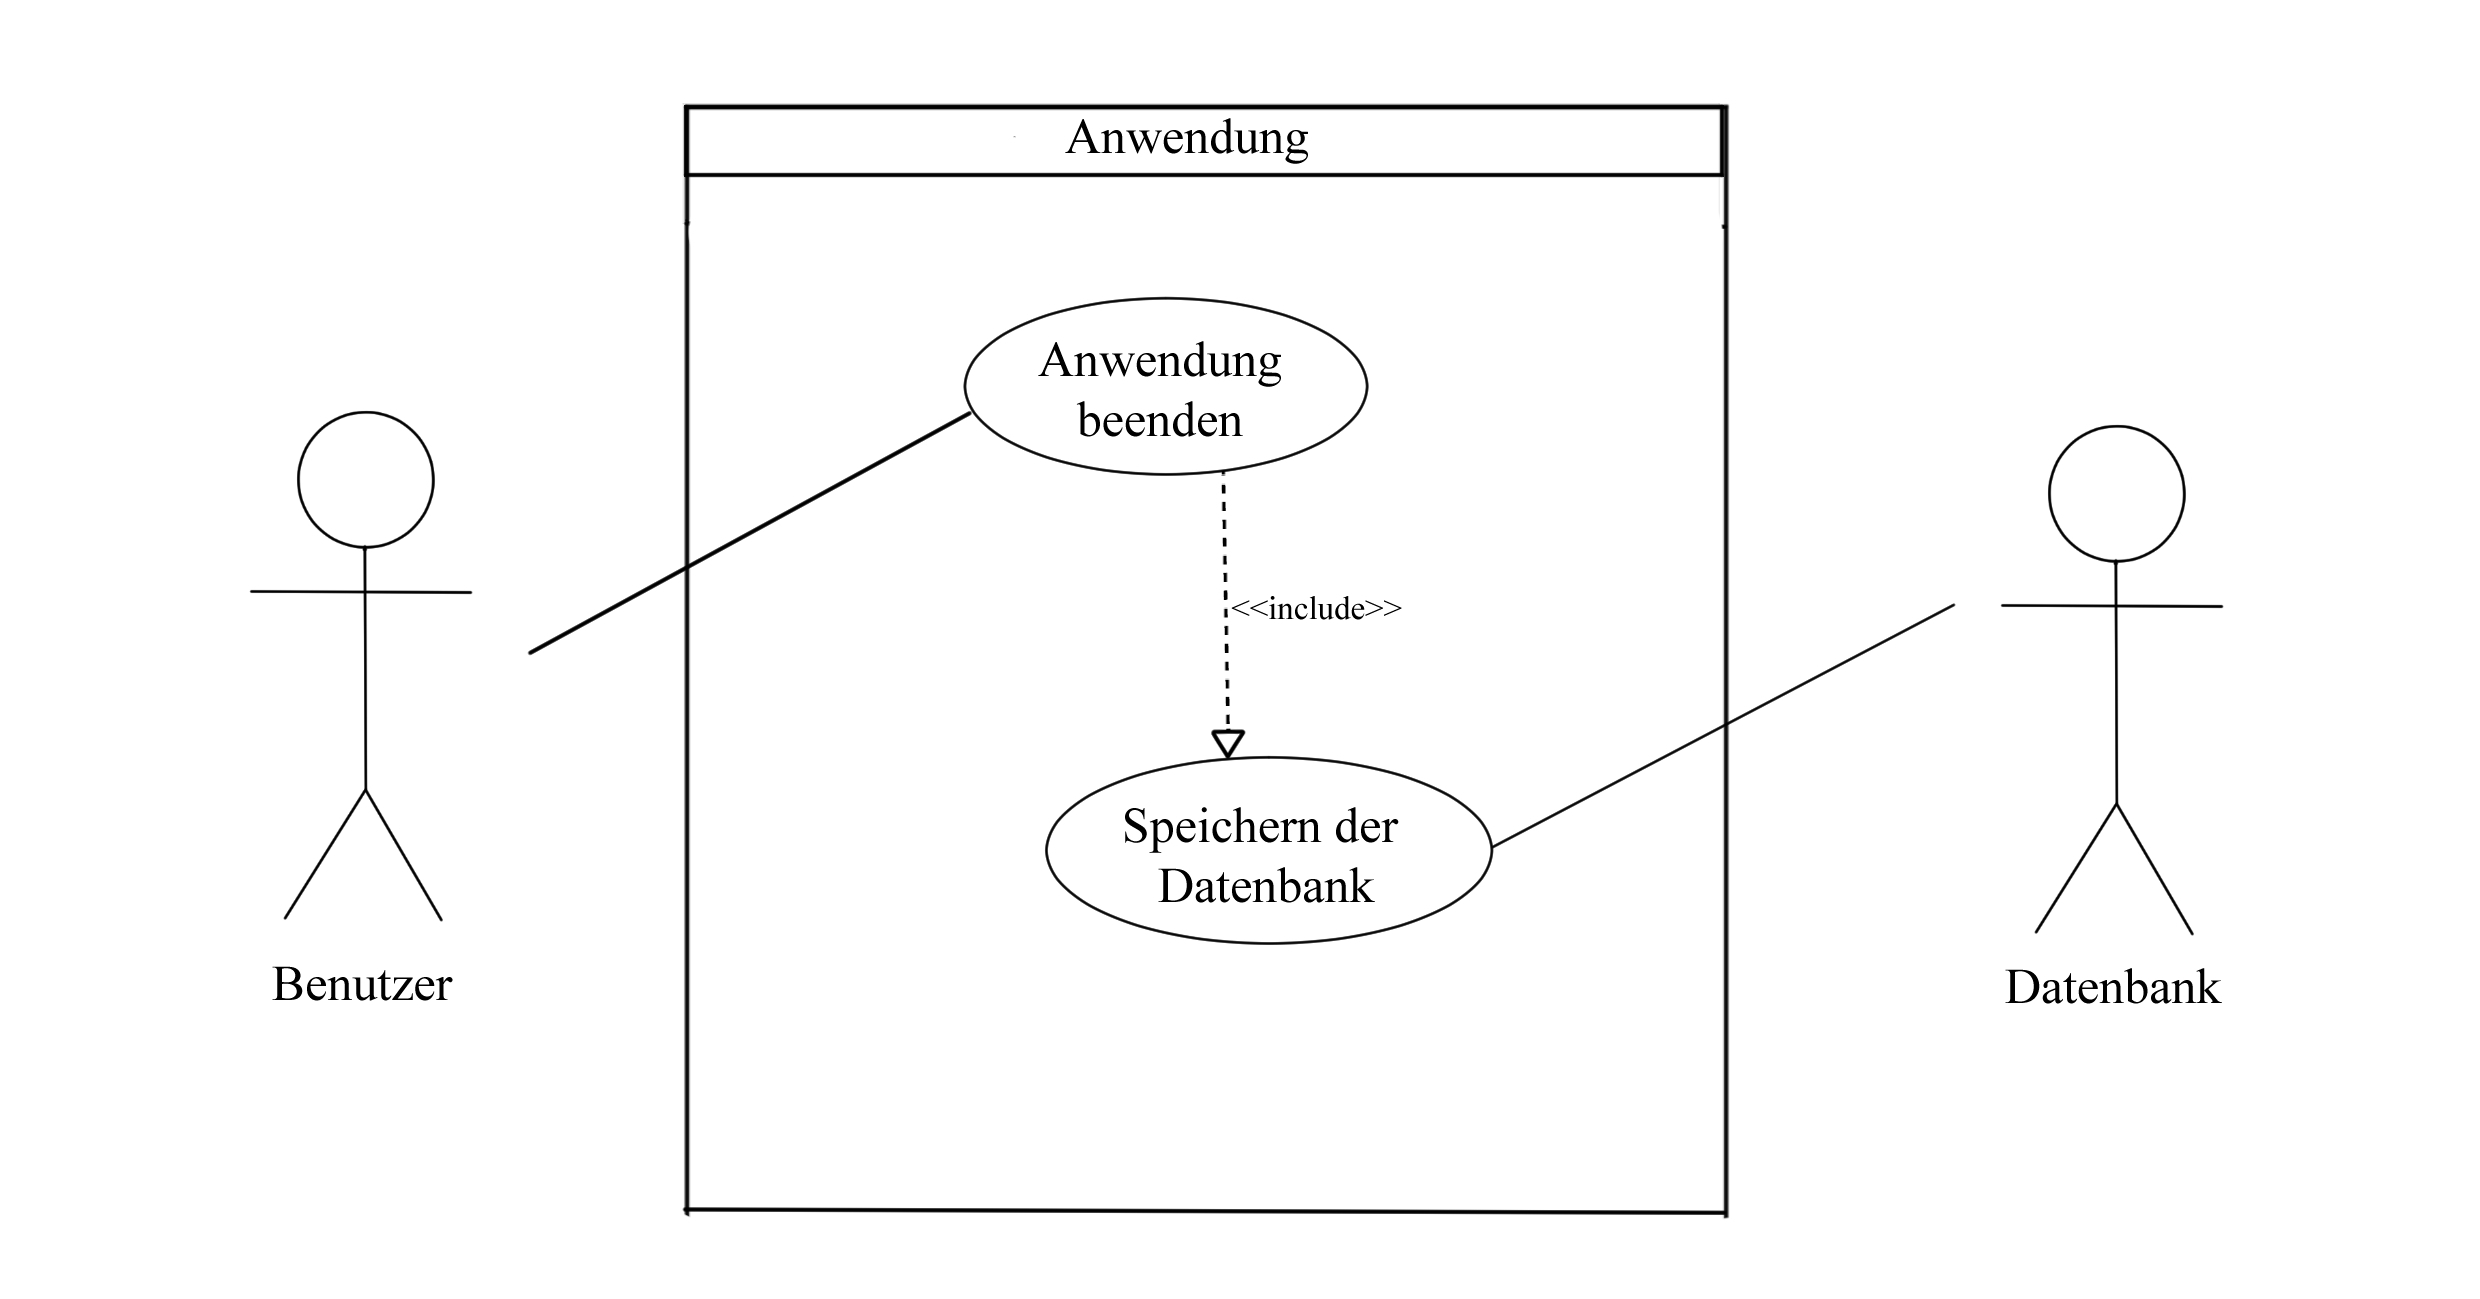
\includegraphics[scale=0.75]{Anwendung_schliessen.jpg}
\centering Abbildung 1: Anwendung schließen
\\
\ \\

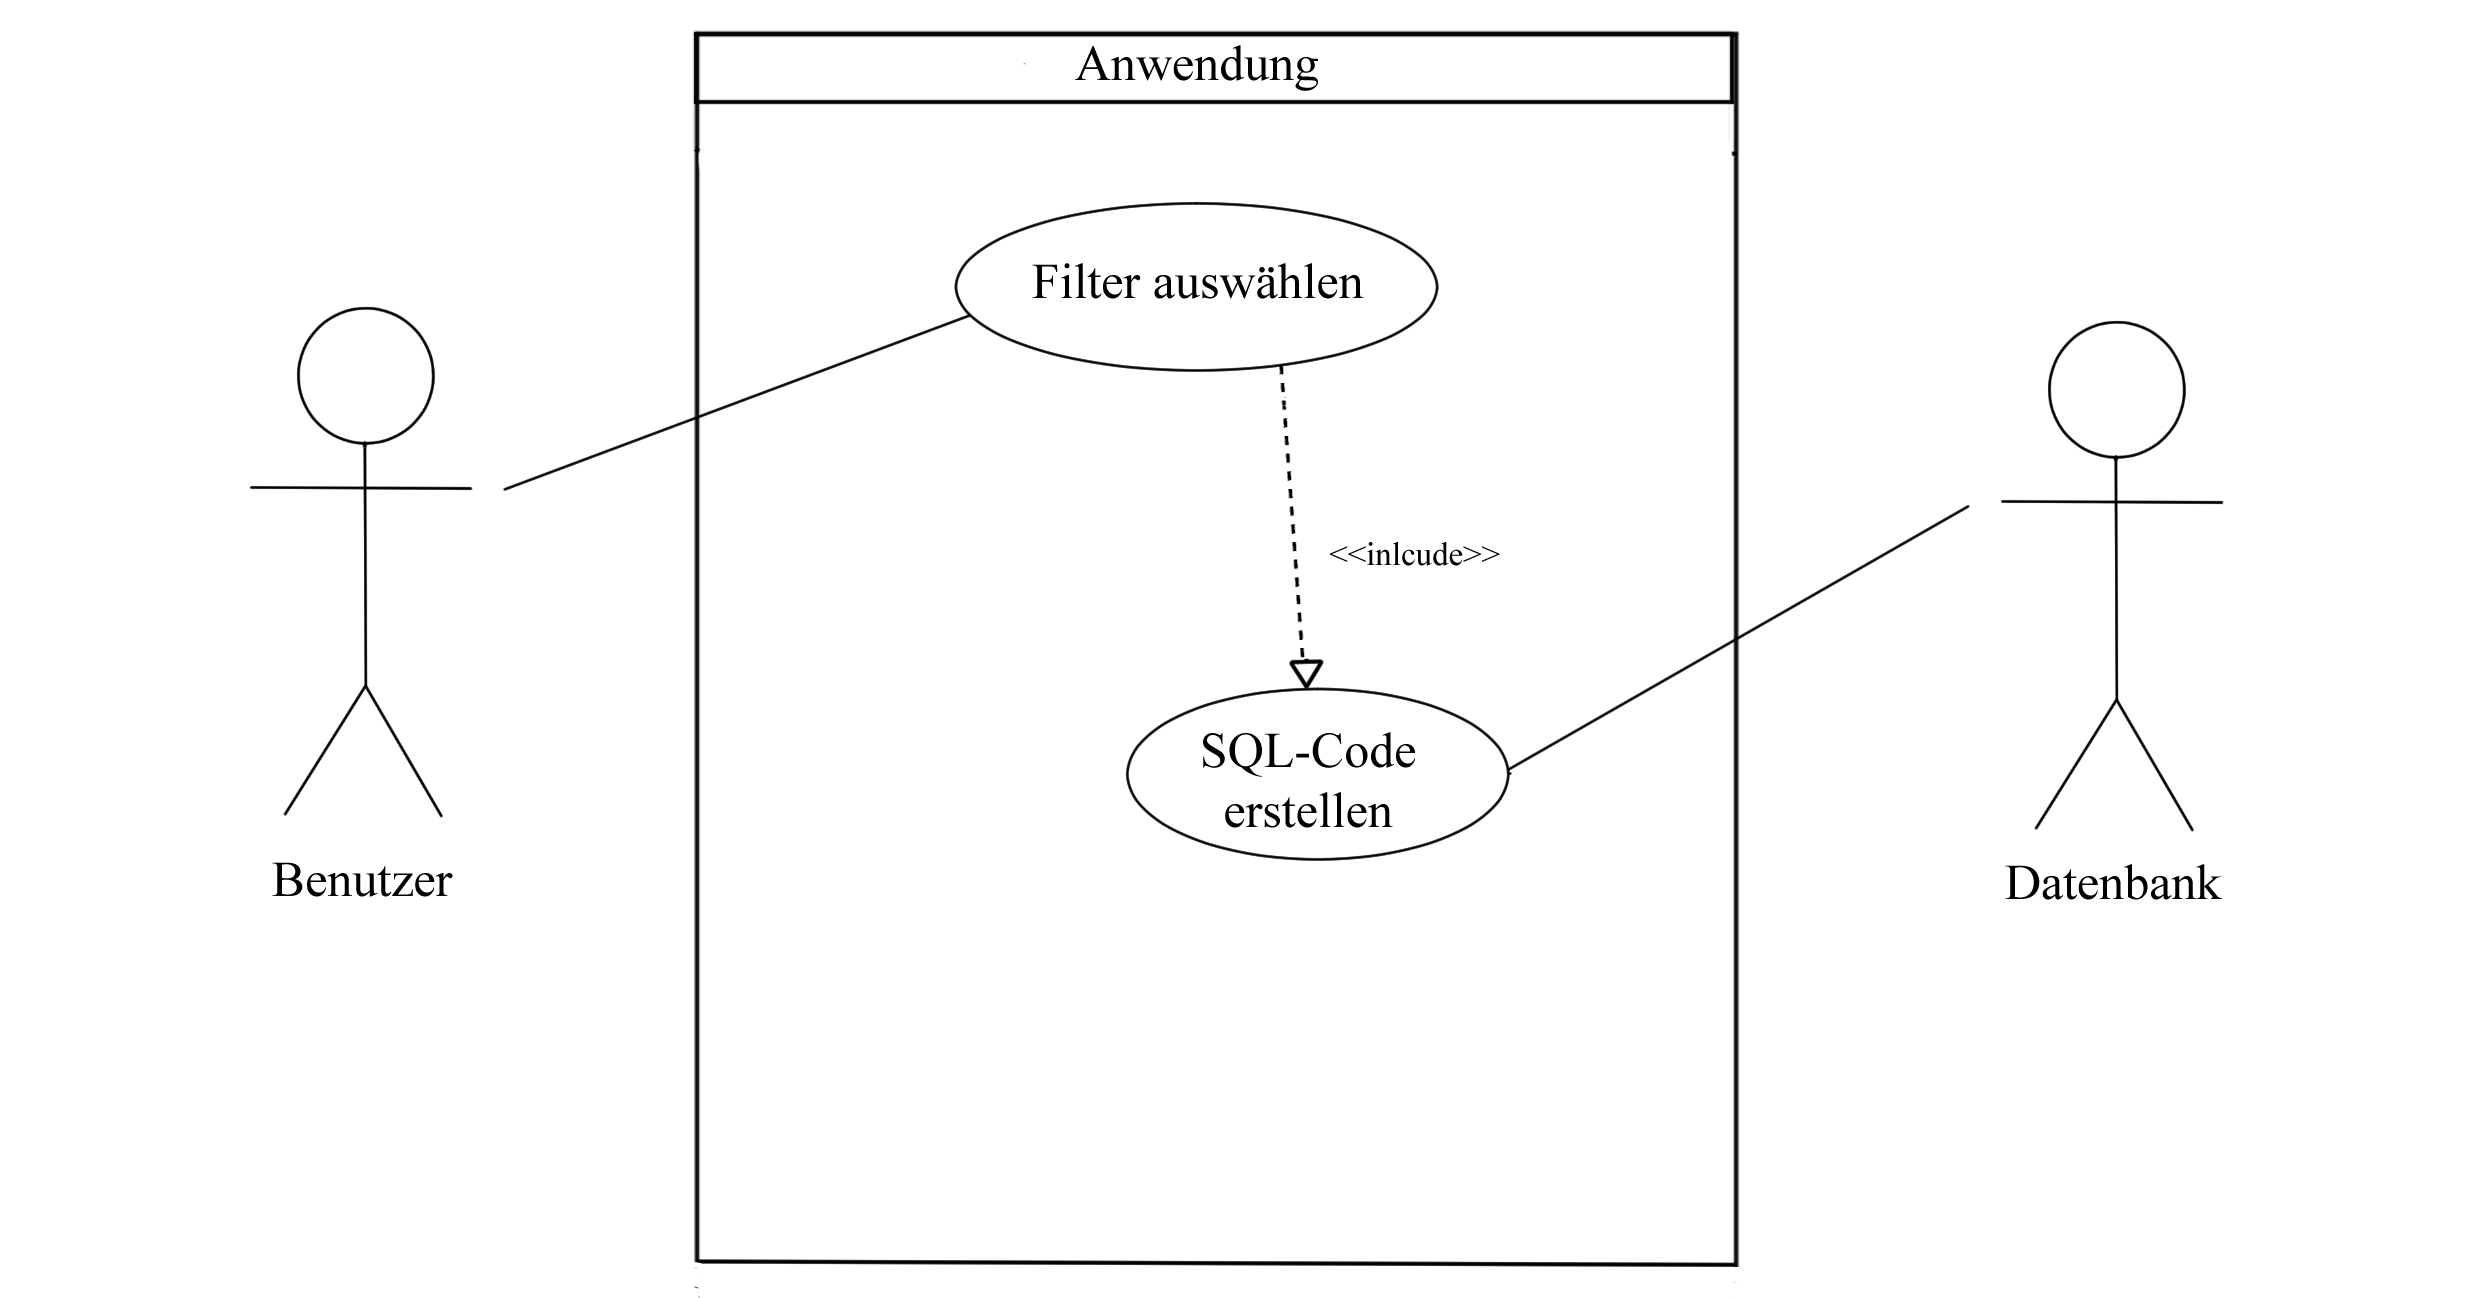
\includegraphics[scale=0.75]{Filter_auswaehlen.jpg}
\centering Abbildung 2: Filter für Graphen auswählen
\\
\ \\

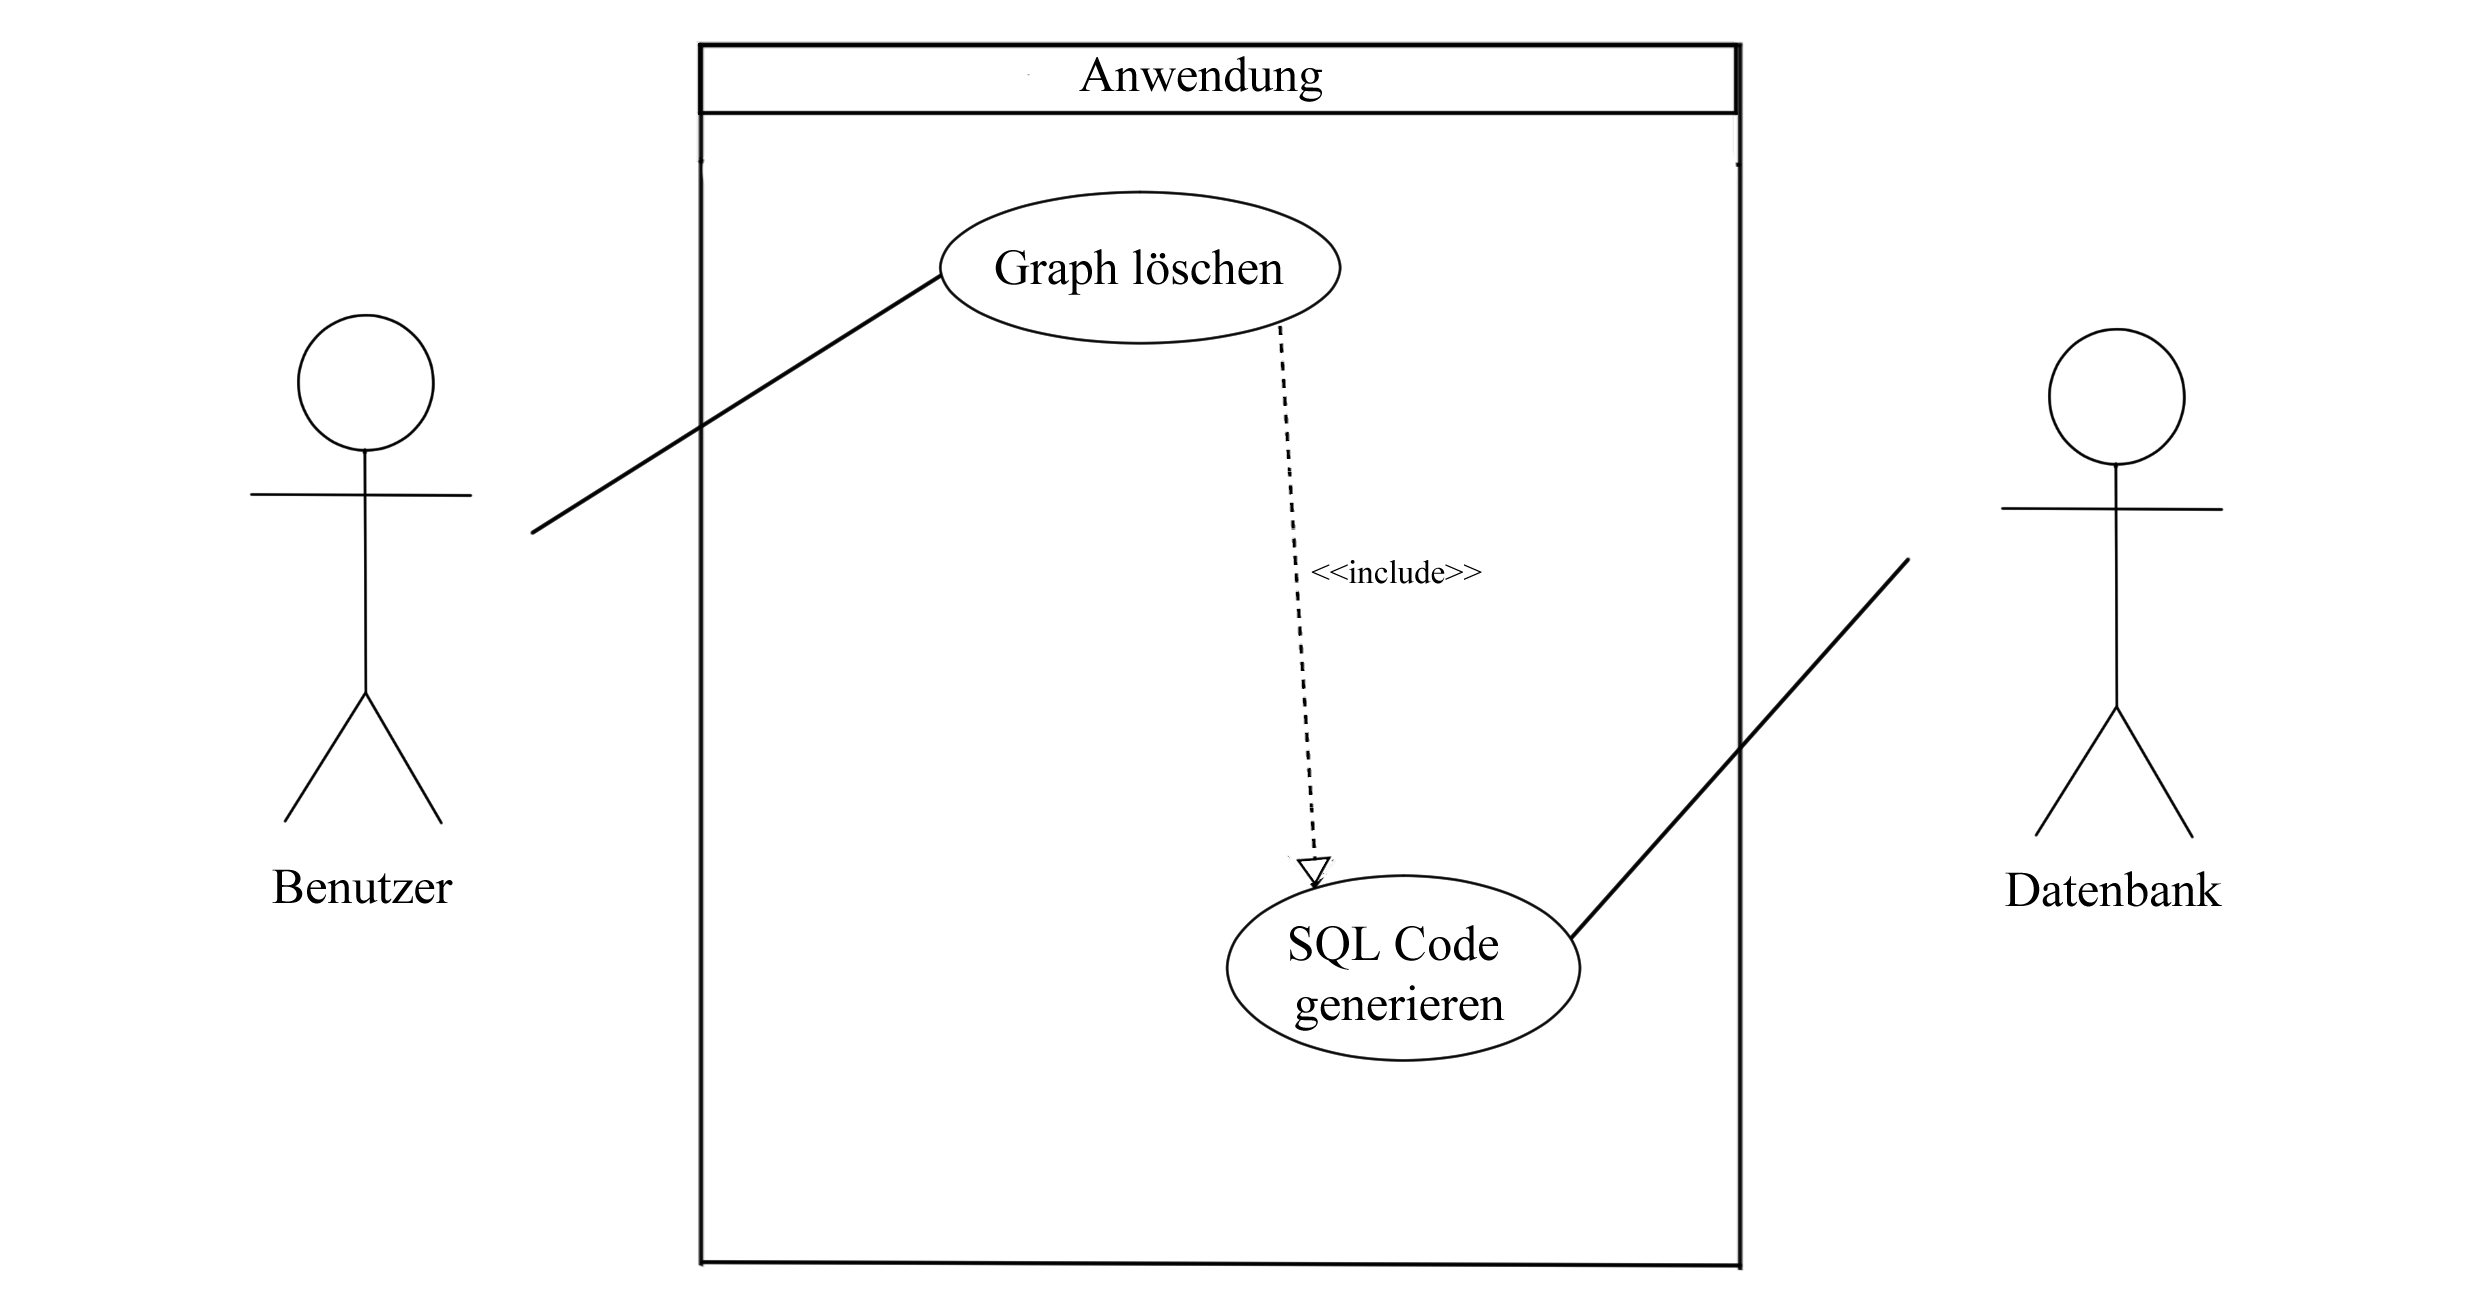
\includegraphics[scale=0.75]{Graph_loeschen.jpg}
\centering Abbildung 3: Ausgewählten Graph löschen
\\
\ \\

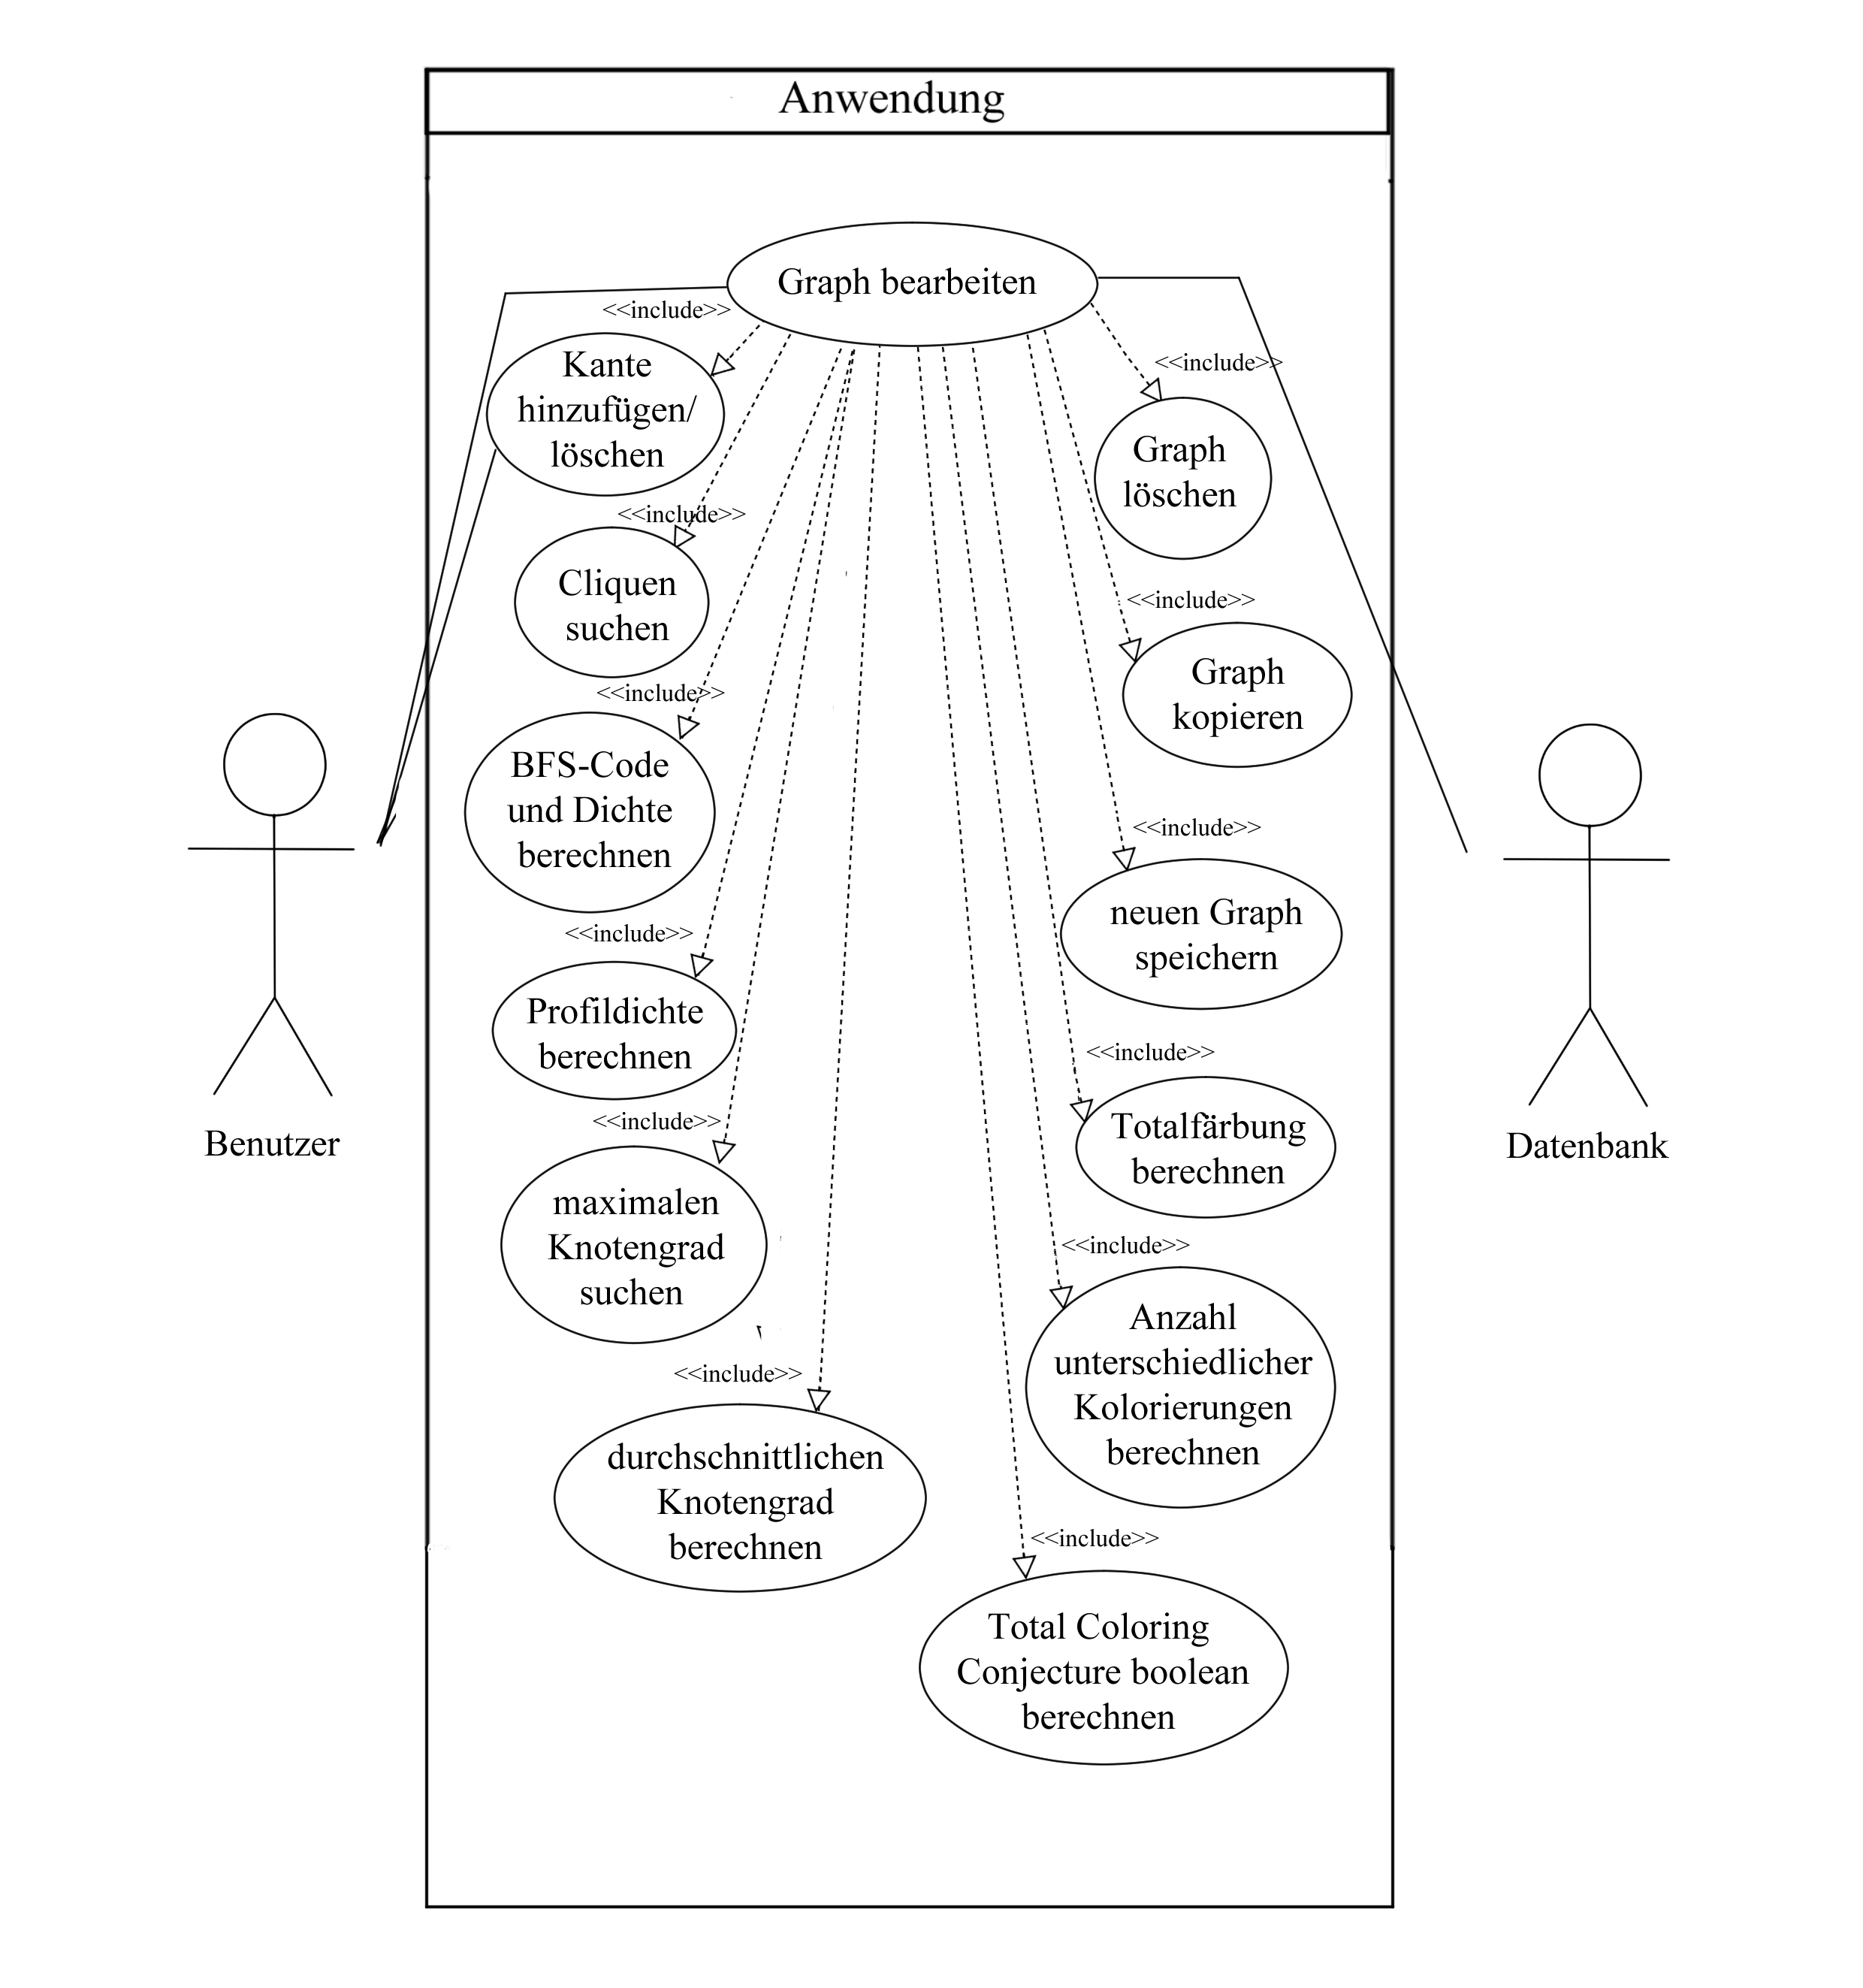
\includegraphics[scale=0.75]{Graph_bearbeiten.jpg}
\centering Abbildung 4: Ausgewählten Graph bearbeiten
\\
\newpage
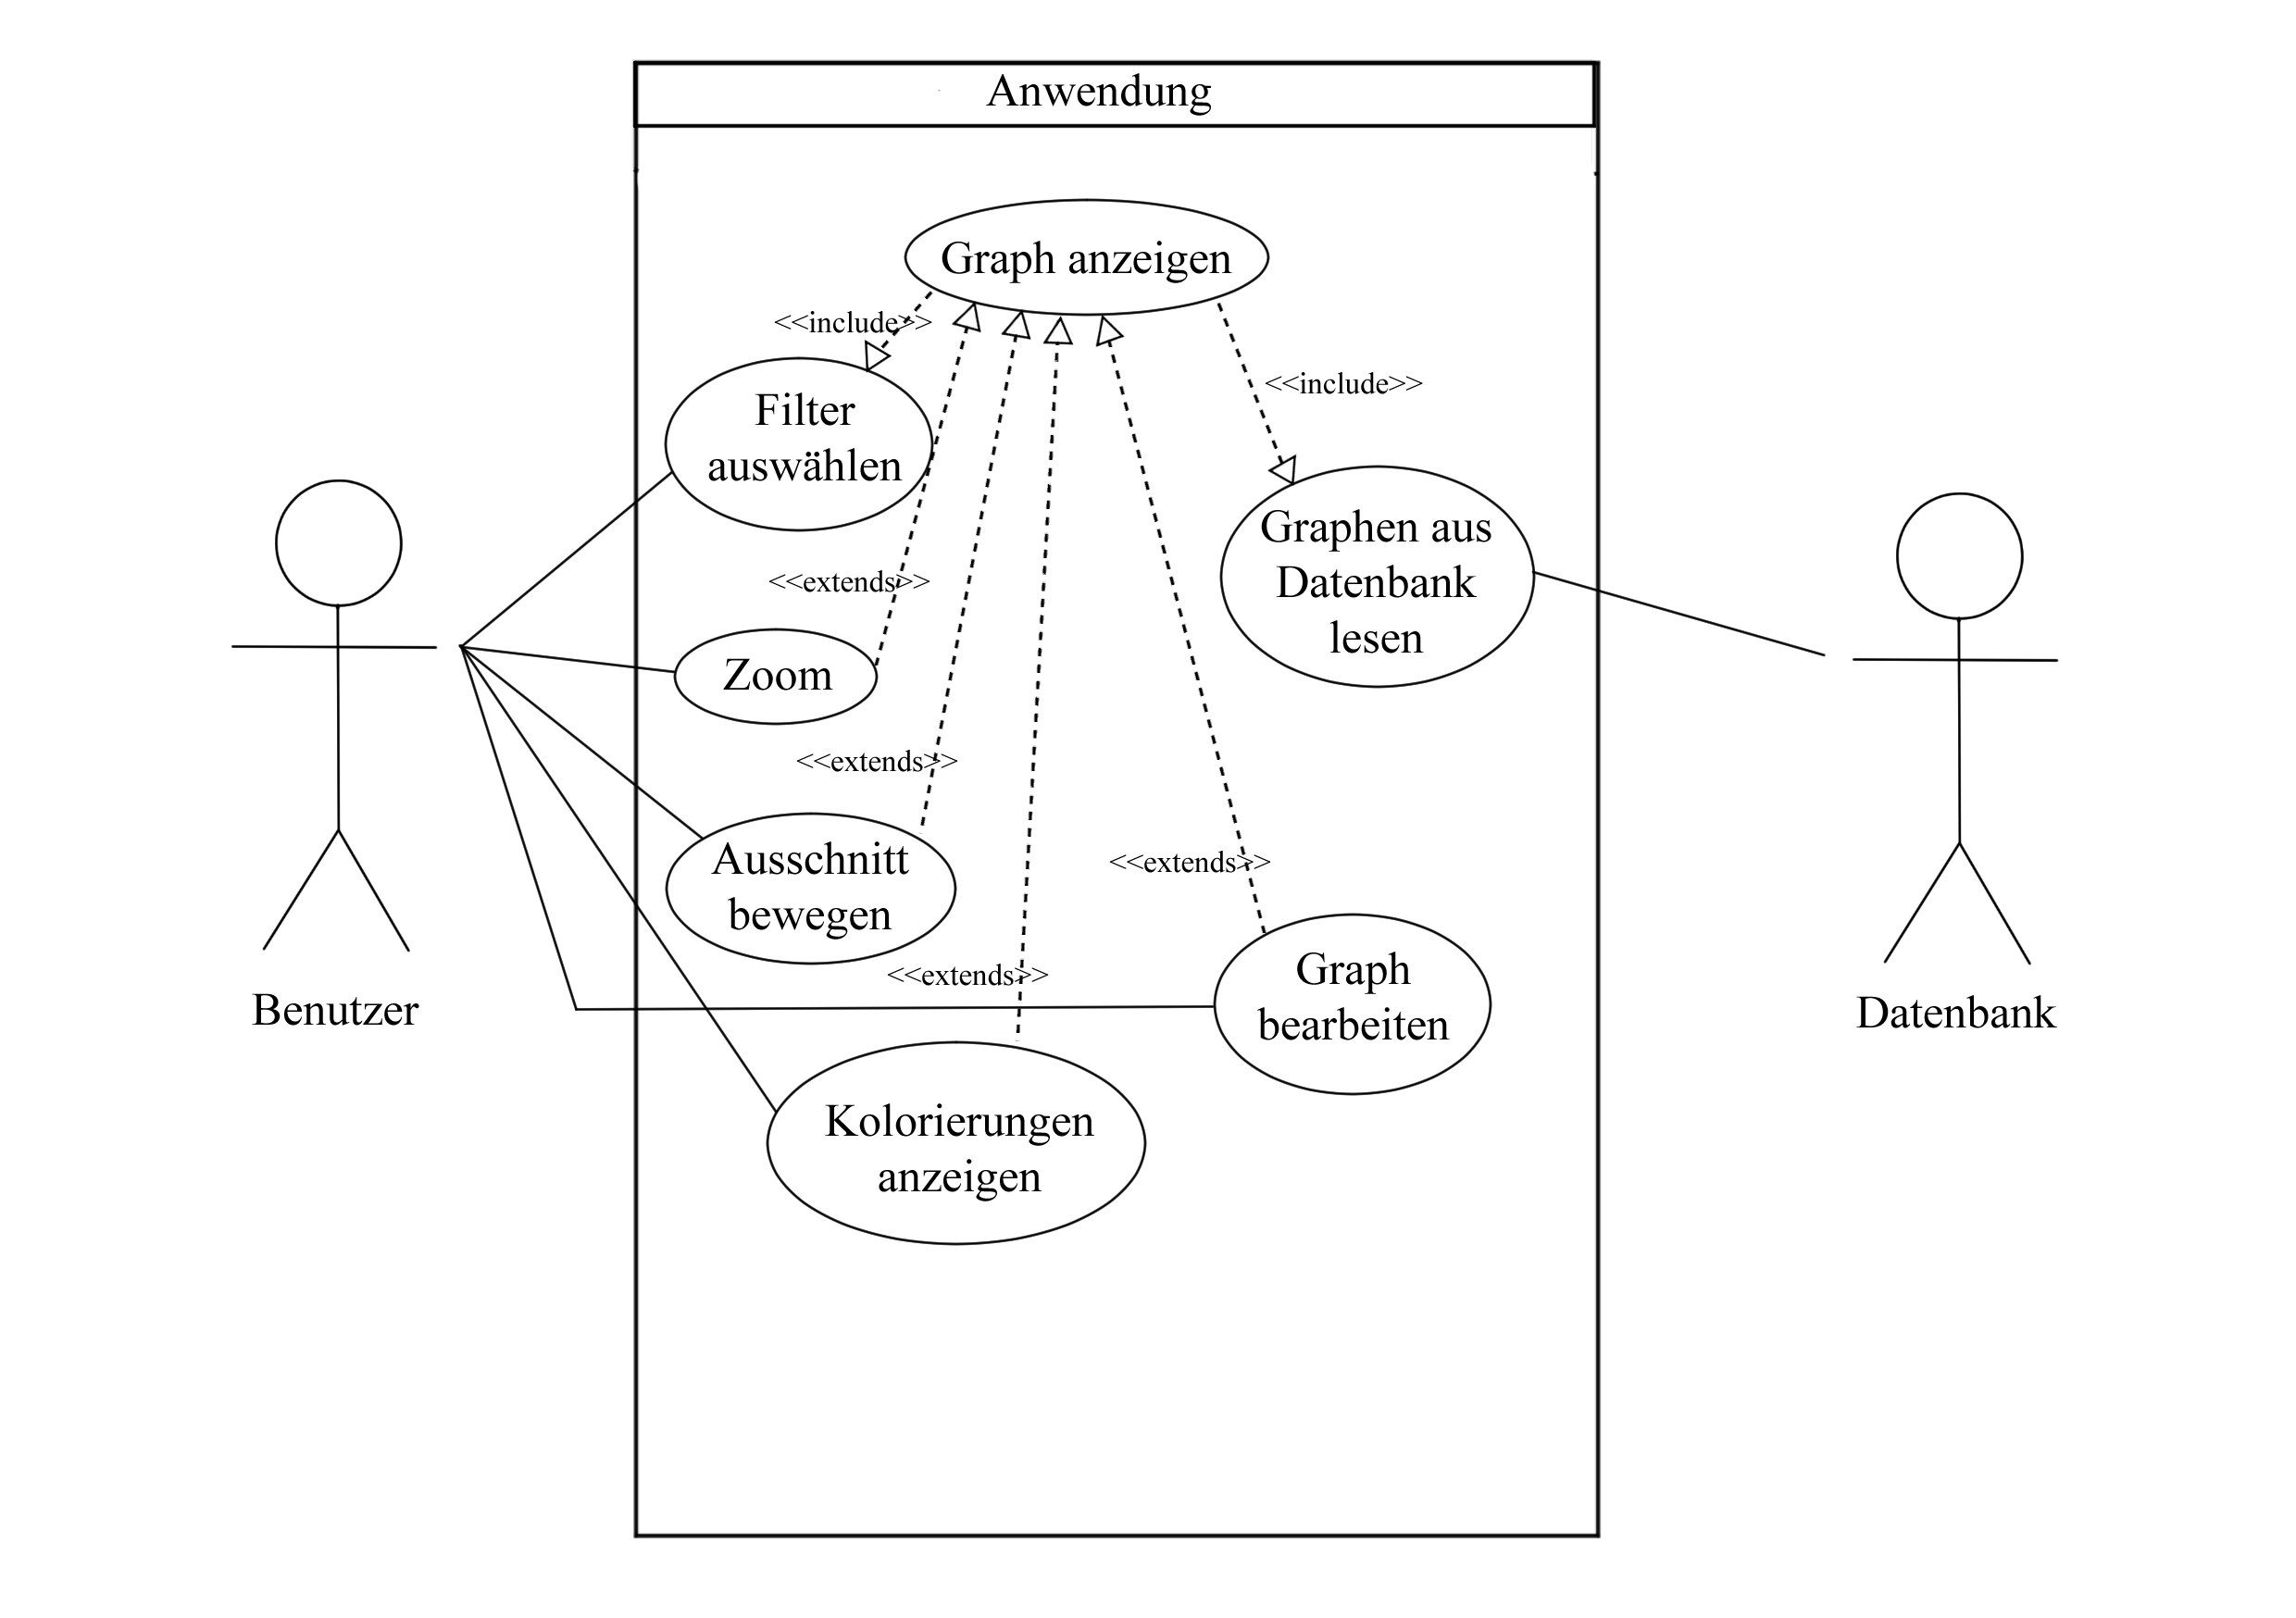
\includegraphics[scale=0.75]{Graph_anzeigen.jpg}
\centering Abbildung 5: den Filtern entsprechende Graphen und ihre Kolorierungen anzeigen
\\

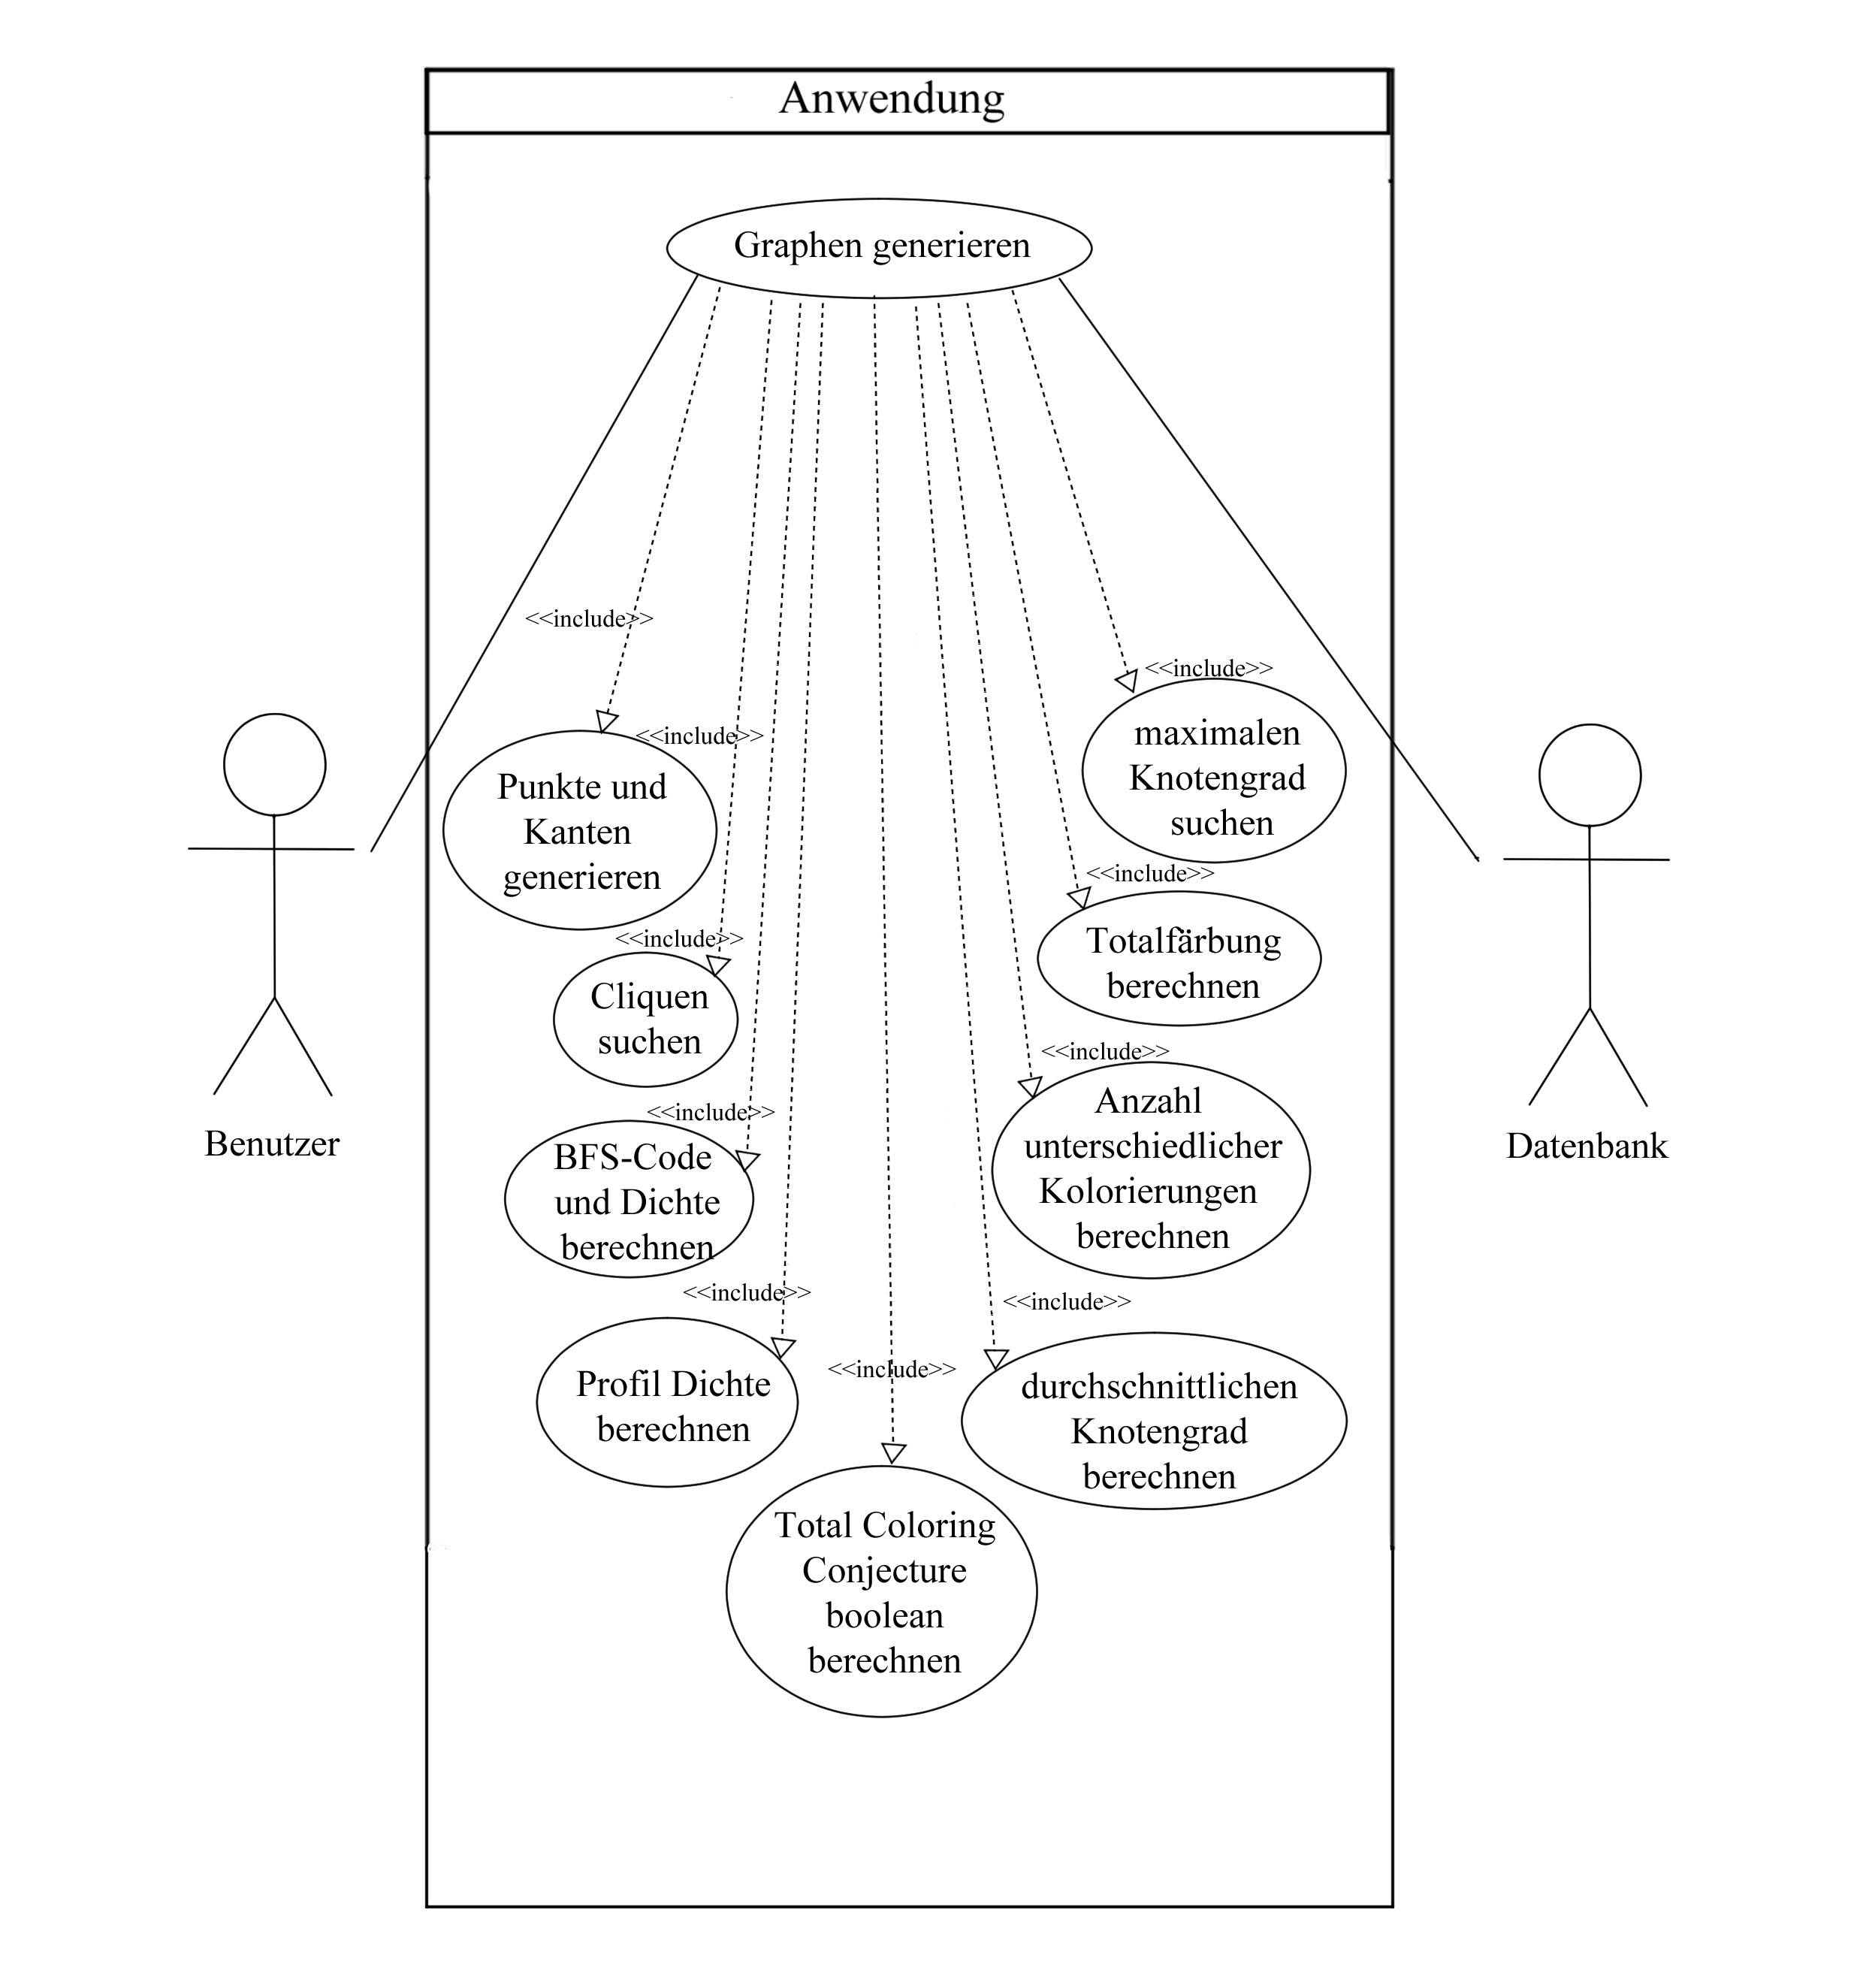
\includegraphics[scale=0.75]{Graphen_generieren.jpg}
\centering Abbildung 6: Ein neues Set Graphen generieren 
\\


\chapter{Benutzeroberfläche}

\begin{flushleft}
Die Benutzeroberfläche ist nach dem bekannten IDE-Konzept aufgebaut, damit die Anwendung auch für neue Benutzer intuitiv bedienbar ist. Sie besteht also aus einem Fenster, welches in vier Abschnitte aufgeteilt ist. Hierbei schließen zwei, über die gesamte Höhe des Fensters reichende Teile, den größten Mittelteil und einen kleineren, darunter liegenden Teil ein. Auf der linken Seite des Fensters befindet sich eine Liste der generierten Graphen, welche die aktiven Filter erfüllen und in einem zweiten Reiter die Konfiguration der Filter. In der Mitte wird, falls ausgewählt, ein Graph visualisiert. Auf der rechten Seite kann man zwischen zwei Reitern wählen.Über den Ersten steuert man die Graphengenerierung, und der Zweite zeigt Statistiken von dem ausgewählten Graph im Vergleich zu den Graphen in der Datenbank an. Am unteren Fensterrand befindet sich die Textausgabe, um den Benutzer über aktuelle Prozesse zu informieren, und ein zweiter Reiter mit den Merkmalen des angezeigten Graphen.
\end{flushleft}

\section{Benutzerschnittstellen Beschreibung}
\subsection{Musskriterien}
\begin{addmargin}[25pt]{0pt}
\begin{enumerate} [label=B\arabic*00,start=1]
	\item Die Datenbestände, bestehend aus Graphen mitsamt ihren \Glspl{Merkmal}n, sollen erstellt, geladen und gelöscht werden können.
	\item Ein ausgewählter Graph soll angezeigt werden können
	\item Es soll ein ausgewählter Graph nach \ref{FA202} bearbeitet werden können. 
	\item In einer Textausgabe werden dem Benutzer Informationen zu laufenden Prozessen mitgeteilt.
	\item Die GUI soll bis auf Texteingaben mit der Maus bedienbar sein.
\setcounter{tempcounter9}{\value{enumi}}
\end{enumerate}
\end{addmargin}
\addtocounter{tempcounter9}{1}
\subsection{Kannkriterien}
\begin{addmargin}[25pt]{0pt}
\begin{enumerate} [label=B\arabic*00,start=\value{tempcounter9}]
	\item Die Bedienung via Shortcuts ist möglich.
	\item Bei der Graphenübersicht wird die Gesamtzahl aller Graphen in der Datenbank im Verhältnis zur Anzahl der ausgewählten Graphen angezeigt. 
\end{enumerate}
\end{addmargin}



\section{GUI Entwürfe}

\subsection{Skizze 1}
    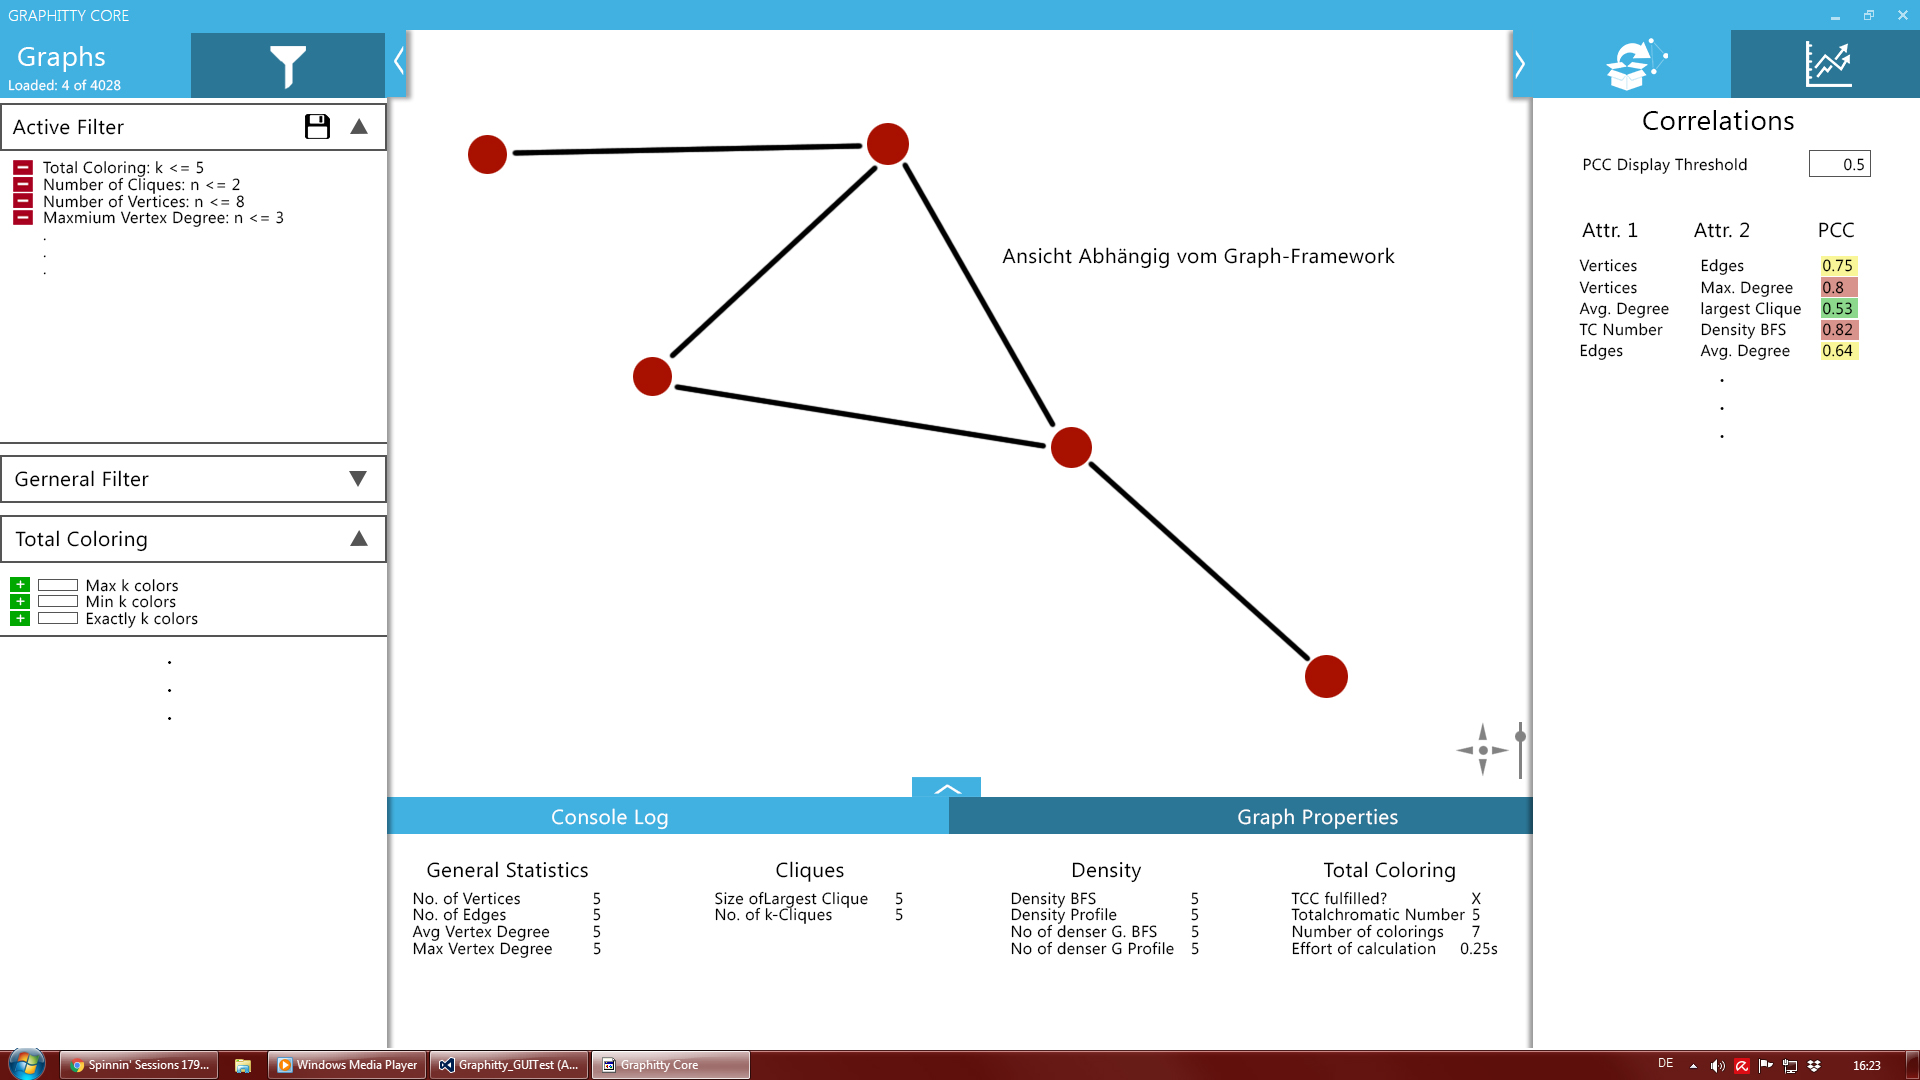
\includegraphics[scale=0.21]{IDE1.jpg}
	\centering Abb. 1: Zeigt die \Glspl{Merkmal} des ausgewählten Graphen an, sowie Filter und Korrelationen.
	\\
\subsection{Skizze 1 - Erklärung}
    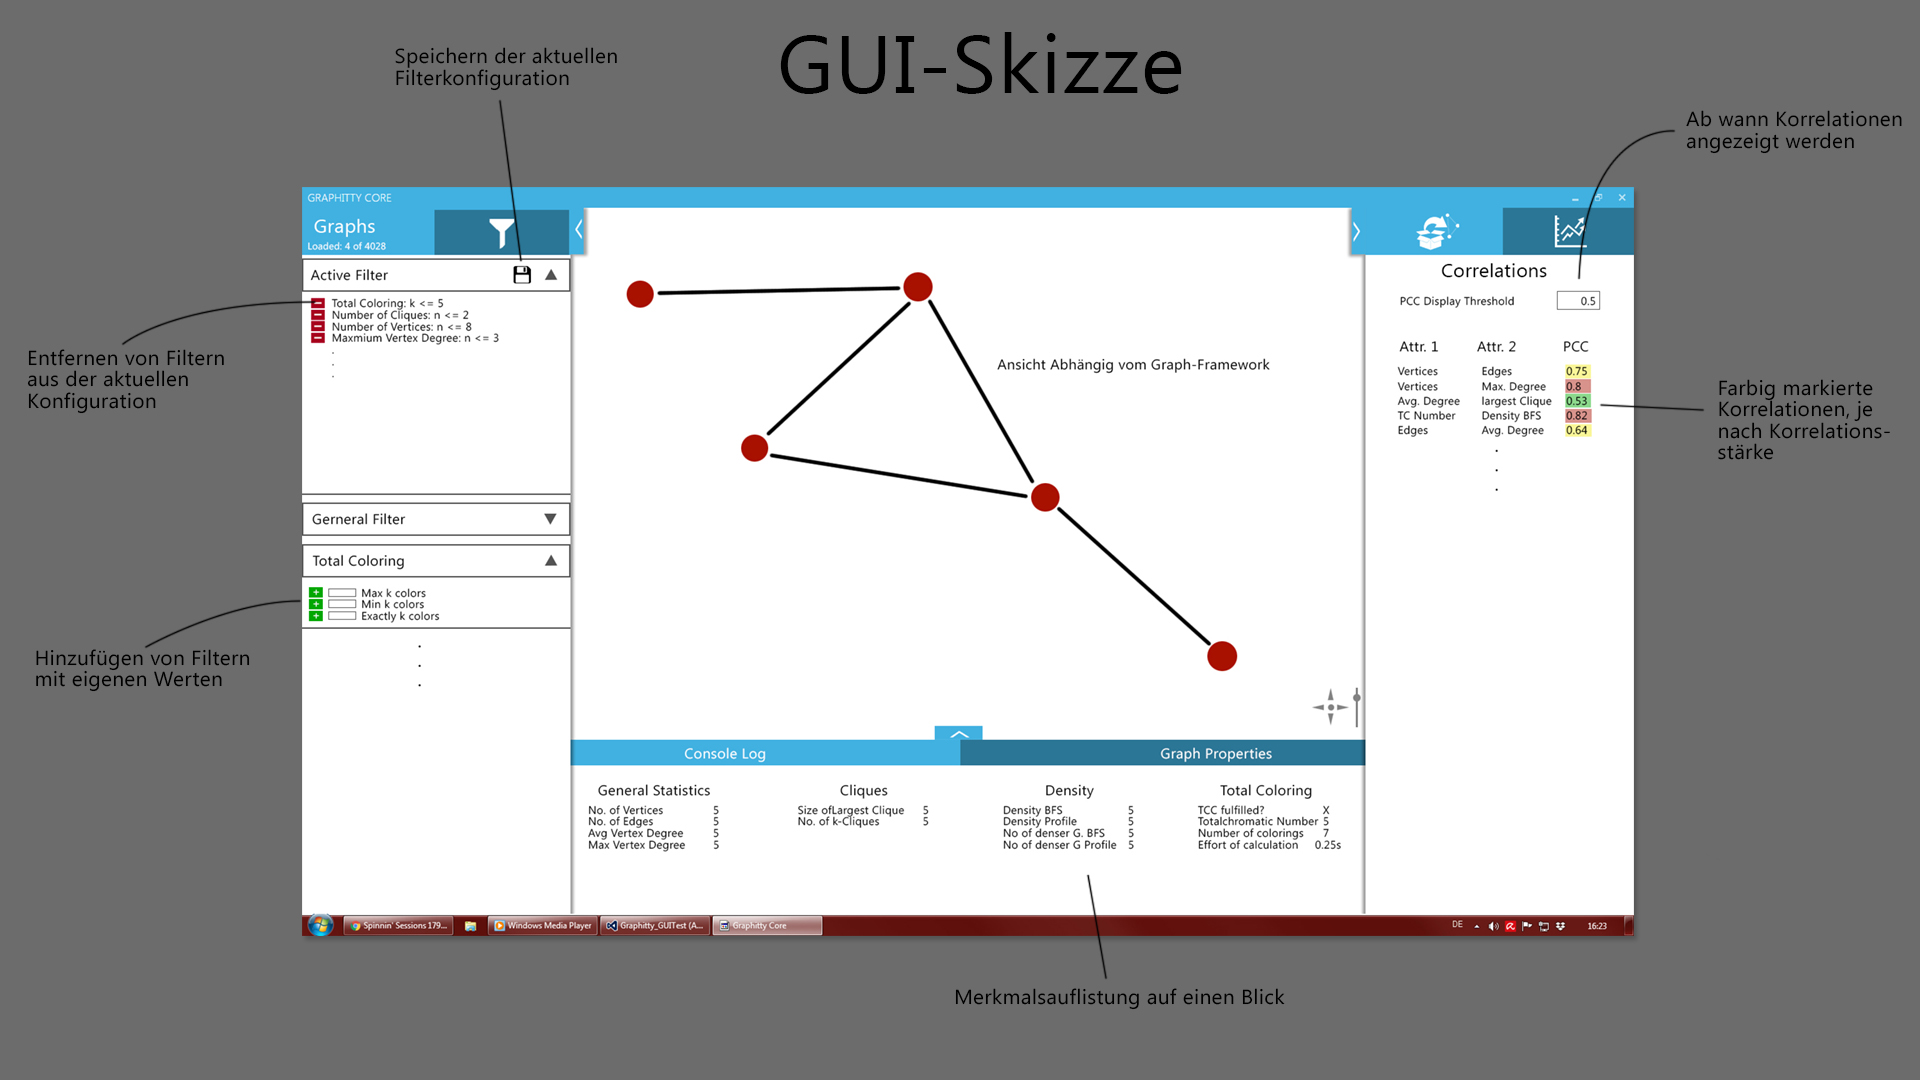
\includegraphics[scale=0.21]{IDE1A.jpg} 
	\centering Abb. 2: Erklärt die Funktionsweise einzelner GUI Elemente.
	\\
\subsection{Skizze 2}
    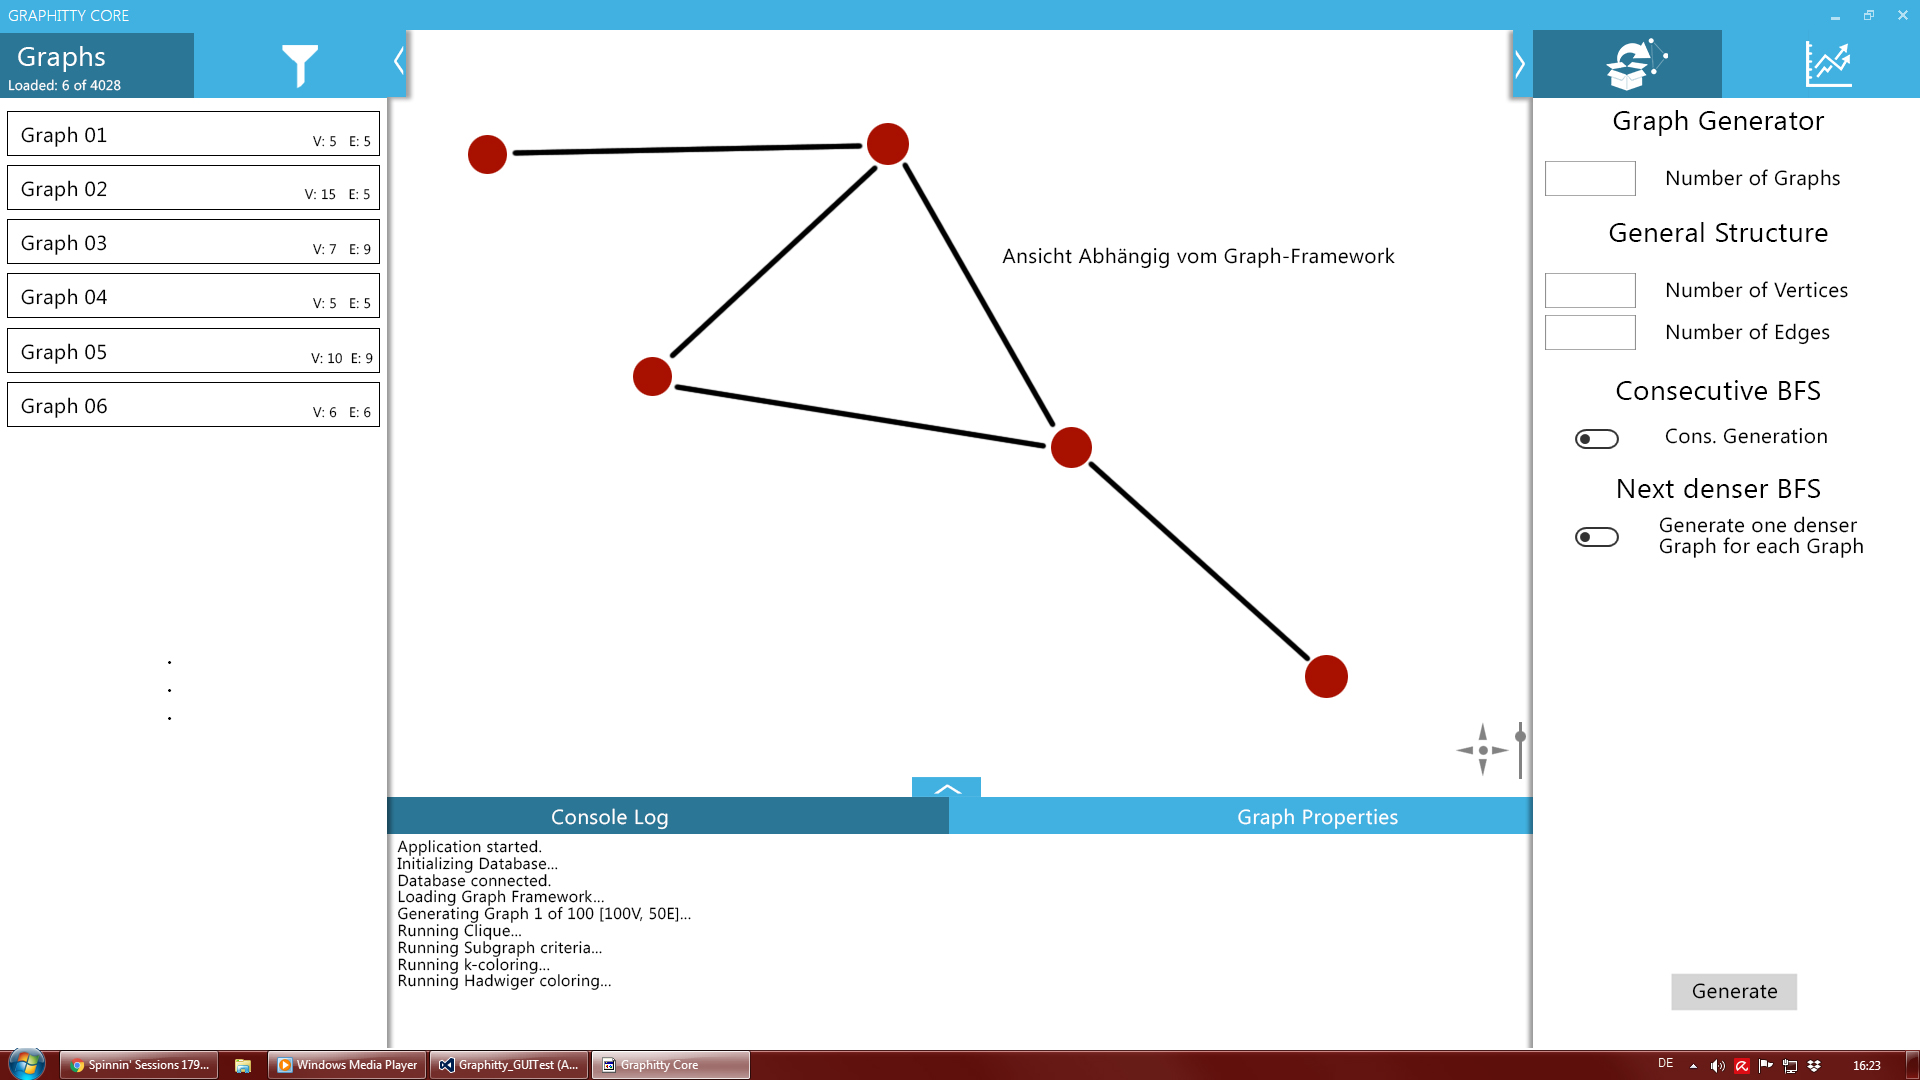
\includegraphics[scale=0.21]{IDE2.jpg}
	\centering Abb. 3: Zeigt die Graphenauflistung, den Graphgenerator und die Textausgabe.
	\\

\chapter{Globale Testfälle}

\subsection{Grundlegende Testfälle}
\begin{flushleft}
Folgend finden sich Testfälle zu den Musskriterien.
\end{flushleft}

\subsubsection{Grundfunktionalität}
\begin{addmargin}[25pt]{0pt}
	\begin{enumerate} [label=T\arabic*,start=100]
		\item Anwendung wird gestartet; (\ref{FA100}):
		\\
		\textbf{Stand:} Anwendung ist nicht gestartet.
		\\
		\textbf{Aktion:} Benutzer startet Anwendung.
		\\
		\textbf{Reaktion:} Die GUI öffnet sich ohne Graphen anzuzeigen.
		
		\item Anwendung wird geschlossen; (\ref{FA101}):
		\\
		\textbf{Stand:} Anwendung funktioniert normal.
		\\
		\textbf{Aktion:} Benutzer schließt die Anwendung ordnungsgemäß.
		\\
		\textbf{Reaktion:} Die Datenbank wird gesichert und die Anwendung terminiert im Anschluss.
	\end{enumerate}
\end{addmargin}

\subsubsection{Datenbank}
\begin{addmargin}[25pt]{0pt}
	\begin{enumerate} [label=T\arabic*,start=200]
		\item Graphenspeicherung; (\ref{FA200}):
		\\
		\textbf{Stand:} Ein Graph wurde generiert und dessen \Glspl{Merkmal} berechnet.
		\\
		\textbf{Aktion:} -
		\\
		\textbf{Reaktion:} Der Graph wird mitsamt ihren \Glspl{Merkmal}n in der Datenbank gespeichert.
		
		\item Löschen eines Graphen; (\ref{FA201}):
		\\
		\textbf{Stand:} Graphen sind generiert und es wird eine Auswahl in der Übersicht dargestellt.
		\\
		\textbf{Aktion:} Benutzer wählt einen Graph zum Löschen aus.
		\\
		\textbf{Reaktion:} Der Graph wird aus der Datenbank entfernt.
		
		\item Bearbeitung von Kanten im Graphen; (\ref{FA202}):
		\\
		\textbf{Stand:} Ein Graph ist ausgewählt und wird angezeigt.
		\\
		\textbf{Aktion:} Benutzer wählt eine Kante zum Löschen aus.
		\\
		\textbf{Reaktion:} Die Kante wird aus dem Graphen entfernt.
		
%		\item Bearbeitung von Knoten im Graphen; (\ref{FA203}):
%		\\
%		\textbf{Stand:} Ein Graph ist ausgewählt und wird angezeigt.
%		\\
%		\textbf{Aktion:} Benutzer wählt einen Knoten zum Löschen aus.
%		\\
%		\textbf{Reaktion:} Der Knoten wird aus dem Graphen entfernt.
%	This Test Case is not needed anymore I think. It has no FA.		
		\item \Glspl{Merkmal} für modifizierten Graphen bestimmen; (\ref{FA203}):
		\\
		\textbf{Stand:} Ein Graph ist ausgewählt und wird angezeigt.
		\\
		\textbf{Aktion:} Benutzer modifiziert Graph nach \ref{FA202} oder \ref{FA203}.
		\\
		\textbf{Reaktion:} \Glspl{Merkmal} des Graphen werden neu berechnet.
		
		\item Speicherung modifizierter Graphen; (\ref{FA204}):
		\\
		\textbf{Stand:} Ein Graph ist modifiziert nach \ref{FA202} oder \ref{FA203}.
		\\
		\textbf{Aktion:} Benutzer wählt die Speichern-Option.
		\\
		\textbf{Reaktion:} Der Graph wird mitsamt seiner \Glspl{Merkmal} in der Datenbank gespeichert.
	\end{enumerate}
\end{addmargin}

\subsubsection{Graphengenerierung}
\begin{addmargin}[25pt]{0pt}
	\begin{enumerate} [label=T\arabic*,start=300]
		\item Graphengenerierung; (\ref{FA300}):
		\\
		\textbf{Stand:} Anwendung ist gestartet.
		\\
		\textbf{Aktion:} Benutzer startet Graphengenerierung.
		\\
		\textbf{Reaktion:} Es werden Graphen mit zufälliger Knotenanzahl und zufälligen Kanten generiert.
	\end{enumerate}
\end{addmargin}

\subsubsection{Grafische Benutzeroberfläche}
\begin{addmargin}[25pt]{0pt}
	\begin{enumerate} [label=T\arabic*,start=400]
		\item Anwenden von \Gls{Filter}n; (\ref{FA401}):
		\\
		\textbf{Stand:} Graphen sind generiert.
		\\
		\textbf{Aktion:} Benutzer wählt \Gls{Filter} aus.
		\\
		\textbf{Reaktion:} Graphen welche die Filterbedingungen erfüllen werden angezeigt.
	\end{enumerate}
\end{addmargin}

\subsubsection{Darstellung der Graphen}
\begin{addmargin}[25pt]{0pt}
	\begin{enumerate} [label=T\arabic*,start=500]
	
		\item Graphen darstellen; (\ref{FA500}):
		\\
		\textbf{Stand:} Graphen sind generiert.
		\\
		\textbf{Aktion:} Benutzer wählt Graphen zur Darstellung aus.
		\\
		\textbf{Reaktion:} Graph wird dargestellt.
		
		\item Darstellung eines Graphen vergrößern und verkleinern; (\ref{FA503}):
		\\
		\textbf{Stand:} Ein Graph wird dargestellt.
		\\
		\textbf{Aktion:} Benutzer zoomt.
		\\
		\textbf{Reaktion:} Darstellung des Graphen ändert sich.
		
		\item Ausschnitt des Graphen bewegen; (\ref{FA504}):
		\\
		\textbf{Stand:} Ein Ausschnitt eines Graphen wird dargestellt.
		\\
		\textbf{Aktion:} Benutzer zieht mit Maus den Graphausschnitt.
		\\
		\textbf{Reaktion:} Der Graphausschnitt bewegt sich in die entsprechende Richtung.
	\end{enumerate}
\end{addmargin}

\subsubsection{Algorithmen}
\subsubsection{Graphengenerierung}
\begin{addmargin}[25pt]{0pt}
	\begin{enumerate} [label=T\arabic*,start=600]
		\item Berechnung der \Glspl{Merkmal} der Graphen; (\ref{FA6}):
		\\
		\textbf{Stand:} Ein Graph wurde generiert.
		\\
		\textbf{Aktion:} -
		\\
		\textbf{Reaktion:} Die Algorithmen berechnen die jeweiligen \Glspl{Merkmal} korrekt.
	\end{enumerate}
\end{addmargin}


\glsaddall
\printnoidxglossaries

\end{document}
